\documentclass[11pt,a4paper]{article}
\usepackage[margin=24mm]{geometry}
\usepackage{amsmath,amssymb,amsthm,bm,graphicx,booktabs,xcolor}
\usepackage[colorlinks=true,linkcolor=blue!50!black,citecolor=blue!50!black,urlcolor=blue!50!black]{hyperref}
\graphicspath{{figures/}}
\setlength{\parskip}{4pt}
\setlength{\parindent}{0pt}
\setlength{\emergencystretch}{2em}
\newcommand{\dd}{\mathrm{d}}
\newcommand{\ii}{\bm i}
\newcommand{\ps}{\bm\psi_s}
\newcommand{\avec}{\bm a}
\newcommand{\bvec}{\bm b}
\newcommand{\norm}[1]{\left\lVert#1\right\rVert}
\newtheorem{proposition}{Proposition}
% Generated by plot_reduction_study.m. All errors in mVs.
\newcommand{\ResultTables}{
\begin{table}[htbp]\centering\small\caption{Set 1: errors on common support. R: reconstruction; P: interior whole-group prediction. Max: largest absolute component error; Q95: vector-error quantile.}\begin{tabular}{llrrrrr}\toprule Method & Mode & RMSE d & RMSE q & Joint & Max & Q95\\\midrule
A & R & 5.239 & 4.041 & 4.678 & 45.87 & 15.66\\
B & R & 4.643 & 3.955 & 4.313 & 32.29 & 13.48\\
C & R & 4.624 & 3.873 & 4.265 & 29.43 & 13.21\\
D & R & 4.626 & 3.876 & 4.267 & 29.46 & 13.28\\
E & R & 4.520 & 3.864 & 4.205 & 29.29 & 12.98\\
F & R & 4.587 & 3.862 & 4.240 & 29.38 & 13.16\\
G & R & 4.474 & 3.956 & 4.223 & 29.70 & 13.19\\
H & R & 0.682 & 0.301 & 0.527 & 4.57 & 1.57\\
A & P & 6.557 & 5.380 & 5.998 & 50.34 & 19.10\\
B & P & 5.927 & 5.223 & 5.586 & 31.29 & 16.87\\
C & P & 5.914 & 5.092 & 5.518 & 31.41 & 16.48\\
D & P & 6.001 & 5.109 & 5.573 & 31.22 & 16.70\\
E & P & 5.785 & 5.099 & 5.453 & 32.75 & 16.60\\
F & P & 5.896 & 5.052 & 5.490 & 30.53 & 16.47\\
G & P & 5.800 & 5.210 & 5.513 & 33.95 & 16.97\\
H & P & 2.362 & 0.898 & 1.787 & 12.09 & 5.68\\
\bottomrule\end{tabular}\par\small Common points: reconstruction 5662/7476; interior prediction 5659/6348.\end{table}
\begin{table}[htbp]\centering\small\caption{Set 2: errors on common support. R: reconstruction; P: interior whole-group prediction. Max: largest absolute component error; Q95: vector-error quantile.}\begin{tabular}{llrrrrr}\toprule Method & Mode & RMSE d & RMSE q & Joint & Max & Q95\\\midrule
A & R & 5.783 & 4.197 & 5.053 & 44.00 & 16.21\\
B & R & 4.936 & 3.958 & 4.474 & 29.08 & 14.30\\
C & R & 5.048 & 3.974 & 4.543 & 29.89 & 14.45\\
D & R & 4.820 & 4.087 & 4.468 & 37.18 & 14.12\\
E & R & 4.726 & 3.974 & 4.366 & 31.32 & 13.76\\
F & R & 4.822 & 3.984 & 4.423 & 29.88 & 13.76\\
G & R & 4.593 & 4.025 & 4.318 & 27.52 & 13.76\\
H & R & 0.719 & 0.316 & 0.556 & 4.28 & 1.77\\
A & P & 7.095 & 5.409 & 6.309 & 45.51 & 20.09\\
B & P & 6.164 & 5.004 & 5.614 & 30.23 & 17.16\\
C & P & 6.369 & 5.024 & 5.736 & 35.54 & 16.98\\
D & P & 6.049 & 5.301 & 5.687 & 30.70 & 17.26\\
E & P & 5.695 & 5.235 & 5.470 & 30.94 & 16.75\\
F & P & 6.201 & 5.047 & 5.653 & 39.65 & 16.92\\
G & P & 5.583 & 5.299 & 5.443 & 33.45 & 16.86\\
H & P & 2.346 & 0.911 & 1.780 & 11.96 & 5.58\\
\bottomrule\end{tabular}\par\small Common points: reconstruction 6175/8092; interior prediction 6175/6936.\end{table}
\begin{table}[htbp]\centering\small\caption{Set 3: errors on common support. R: reconstruction; P: interior whole-group prediction. Max: largest absolute component error; Q95: vector-error quantile.}\begin{tabular}{llrrrrr}\toprule Method & Mode & RMSE d & RMSE q & Joint & Max & Q95\\\midrule
A & R & 5.462 & 5.469 & 5.466 & 34.75 & 16.34\\
B & R & 4.953 & 5.602 & 5.287 & 30.59 & 15.29\\
C & R & 4.880 & 5.605 & 5.255 & 30.05 & 15.24\\
D & R & 4.926 & 5.618 & 5.283 & 30.17 & 15.38\\
E & R & 4.897 & 5.401 & 5.155 & 31.88 & 14.95\\
F & R & 4.820 & 5.173 & 5.000 & 26.68 & 14.87\\
G & R & 4.009 & 5.628 & 4.886 & 26.06 & 14.60\\
H & R & 0.409 & 0.210 & 0.325 & 2.02 & 0.85\\
A & P & 6.899 & 7.041 & 6.970 & 35.94 & 19.93\\
B & P & 6.629 & 7.199 & 6.920 & 33.81 & 18.63\\
C & P & 6.837 & 7.151 & 6.996 & 32.47 & 19.01\\
D & P & 6.328 & 7.080 & 6.714 & 32.82 & 18.40\\
E & P & 6.616 & 7.055 & 6.839 & 32.36 & 18.58\\
F & P & 6.147 & 6.890 & 6.529 & 33.84 & 18.17\\
G & P & 5.580 & 7.171 & 6.425 & 30.91 & 17.84\\
H & P & 1.898 & 0.883 & 1.480 & 8.33 & 3.91\\
\bottomrule\end{tabular}\par\small Common points: reconstruction 6630/9022; interior prediction 6592/7264.\end{table}
}
\newcommand{\FactorTable}{\begin{tabular}{lrrrr}\toprule Set & A & B & C & Derivative LS\\\midrule
1 & 13.4921 & 14.2412 & 14.3385 & 13.8374\\
2 & 13.5184 & 14.3506 & 14.1803 & 13.9514\\
3 & 14.7642 & 14.0315 & 13.9320 & 14.4482\\
\bottomrule\end{tabular}}
\newcommand{\ParameterTable}{\begin{tabular}{llrrrrr}\toprule Set & Method & $c_1$ & $c_2$ & $c_3$ & $c_4$ & $c_5$\\\midrule
1 & D & 14.3467 & -0.0105 & NaN & NaN & NaN\\
1 & E & 14.4339 & -0.0381 & -0.2185 & NaN & NaN\\
1 & F & 14.3367 & -0.0256 & NaN & NaN & NaN\\
1 & G & 14.0170 & 0.1052 & -0.6091 & 0.4575 & 0.5941\\
2 & D & 14.9016 & -0.9459 & NaN & NaN & NaN\\
2 & E & 14.7639 & -0.3724 & -0.1483 & NaN & NaN\\
2 & F & 14.1870 & -0.0918 & NaN & NaN & NaN\\
2 & G & 14.1210 & -0.2569 & -0.4607 & -0.0279 & 1.0622\\
3 & D & 14.0365 & -0.1092 & NaN & NaN & NaN\\
3 & E & 14.0883 & 0.0256 & 1.2640 & NaN & NaN\\
3 & F & 14.6271 & -0.7879 & NaN & NaN & NaN\\
3 & G & 15.0134 & -1.2991 & 0.0466 & -0.2755 & 1.5915\\
\bottomrule\end{tabular}}
\newcommand{\DerivativeTable}{\begin{tabular}{lrrrrr}\toprule Set & $k_{\rm LS}$ & median $\eta$ & $\rho_A$ & $\rho_{LS}$ & $\rho_{local}$\\\midrule
1 & 13.837 & 0.090 & 0.162 & 0.160 & 0.088\\
2 & 13.951 & 0.087 & 0.156 & 0.153 & 0.083\\
3 & 14.448 & 0.144 & 0.197 & 0.196 & 0.138\\
\bottomrule\end{tabular}}
\newcommand{\SurfaceTable}{\begin{tabular}{lrrrrrrr}\toprule Set & A & B & C & D & E & F & G\\\midrule
1 & 1.868 & 1.841 & 1.853 & 1.852 & 1.844 & 1.852 & 1.800\\
\multicolumn{8}{l}{Common pair anchors: 13906/14677.}\\
2 & 1.820 & 1.801 & 1.784 & 1.774 & 1.782 & 1.787 & 1.751\\
\multicolumn{8}{l}{Common pair anchors: 15076/15927.}\\
3 & 2.597 & 2.642 & 2.661 & 2.650 & 2.625 & 2.542 & 2.422\\
\multicolumn{8}{l}{Common pair anchors: 10848/11712.}\\
\bottomrule\end{tabular}}
\newcommand{\NumericalTable}{\begin{tabular}{llrrr}\toprule Set & Control & RMSE d & RMSE q & Points\\\midrule
1 & A normalized & 5.244 & 4.039 & 5625\\
1 & A raw axes & 5.341 & 4.089 & 5625\\
1 & H normalized & 0.683 & 0.301 & 5625\\
1 & H raw axes & 0.771 & 0.363 & 5625\\
1 & A raster 41 & 6.716 & 5.527 & 7129\\
1 & A raster 81 & 5.628 & 4.406 & 7129\\
1 & A raster 161 & 4.356 & 3.236 & 7129\\
2 & A normalized & 5.796 & 4.195 & 6131\\
2 & A raw axes & 5.836 & 4.192 & 6131\\
2 & H normalized & 0.721 & 0.316 & 6131\\
2 & H raw axes & 0.861 & 0.394 & 6131\\
2 & A raster 41 & 7.114 & 5.501 & 7729\\
2 & A raster 81 & 6.279 & 4.498 & 7729\\
2 & A raster 161 & 4.622 & 3.241 & 7729\\
3 & A normalized & 5.363 & 5.456 & 6607\\
3 & A raw axes & 5.370 & 5.459 & 6607\\
3 & H normalized & 0.409 & 0.210 & 6607\\
3 & H raw axes & 0.762 & 0.418 & 6607\\
3 & A raster 41 & 6.533 & 6.657 & 8667\\
3 & A raster 81 & 5.837 & 5.934 & 8667\\
3 & A raster 161 & 4.384 & 4.264 & 8667\\
\bottomrule\end{tabular}}
\newcommand{\ContourTable}{\begin{tabular}{lrrr}\toprule Set & $k_A$ & Centroid RMS in mVs & median $|\Delta i_q/\Delta i_e|$\\\midrule
1 & 13.4921 & 29.223 & 2.547\\
2 & 13.5184 & 28.854 & 3.712\\
3 & 14.7642 & 14.176 & 4.706\\
\bottomrule\end{tabular}}
\newcommand{\SensitivityTable}{\begin{tabular}{lrrr}\toprule Set & Neighbours & Derivative LS & $\rho$\\\midrule
1 & 40 & 13.9539 & 0.1538\\
1 & 80 & 13.8831 & 0.1473\\
1 & 120 & 13.7939 & 0.1464\\
2 & 40 & 14.1177 & 0.1461\\
2 & 80 & 14.0148 & 0.1428\\
2 & 120 & 13.9344 & 0.1422\\
3 & 40 & 14.5383 & 0.1867\\
3 & 80 & 14.5119 & 0.1819\\
3 & 120 & 14.4667 & 0.1801\\
\bottomrule\end{tabular}}
\newcommand{\NominalTable}{\begin{tabular}{lrrr}\toprule Set & RMS d in mVs & RMS q in mVs & Points\\\midrule
1 & 2.042 & 1.014 & 5662\\
2 & 2.024 & 0.977 & 6175\\
3 & 2.556 & 1.577 & 6630\\
\bottomrule\end{tabular}}
\newcommand{\OptimizerTable}{\begin{tabular}{lrrrrrrr}\toprule Set & B & C & D & E & F & G & Runs/model\\\midrule
1 & 0 & 0 & 0 & 0 & 0 & 2 & 14\\
2 & 0 & 0 & 0 & 0 & 0 & 1 & 15\\
3 & 0 & 0 & 0 & 0 & 0 & 1 & 11\\
\bottomrule\end{tabular}}
\newcommand{\BoundaryTable}{\begin{tabular}{lrlrrr}\toprule Set & Excitation & Method & Joint in mVs & Points & Coverage\\\midrule
1 & 2 & C & 7.142 & 509 & 0.881\\
1 & 2 & G & 7.187 & 509 & 0.881\\
1 & 2 & H & NaN & 0 & 0.000\\
1 & 40 & C & 11.127 & 455 & 0.827\\
1 & 40 & G & 11.986 & 455 & 0.827\\
1 & 40 & H & NaN & 0 & 0.000\\
2 & 0 & C & 6.554 & 515 & 0.891\\
2 & 0 & G & 7.475 & 515 & 0.891\\
2 & 0 & H & NaN & 0 & 0.000\\
2 & 40 & C & 13.336 & 465 & 0.804\\
2 & 40 & G & 10.981 & 465 & 0.804\\
2 & 40 & H & NaN & 0 & 0.000\\
3 & 3 & C & 10.238 & 811 & 0.874\\
3 & 3 & G & 9.568 & 811 & 0.874\\
3 & 3 & H & NaN & 0 & 0.000\\
3 & 30 & C & 11.805 & 723 & 0.871\\
3 & 30 & G & 11.115 & 723 & 0.871\\
3 & 30 & H & NaN & 0 & 0.000\\
\bottomrule\end{tabular}}

\title{\Large Mathematical Derivation and Experimental Validation\\of Excitation-Current Coordinate Reduction\\in Electrically Excited Synchronous Machines}
\author{Winding Factor Research Study}
\date{23 October 2026}
\begin{document}
\maketitle
\begin{abstract}
The replacement \(s=i_d+k i_e\) is examined as a reduction of the two stator flux-linkage functions of an electrically excited synchronous machine. Starting from the supplied handwritten derivation, we distinguish constant-flux secants, differential slope ratios, local proportionality of coupling vectors, and a globally constant shift. A common constant-factor reduction requires \(L_{de}=kL_{dd}\) and \(L_{qe}=kL_{qd}\). A normalized determinant and a joint least-squares factor quantify departures without dividing by a small cross-inductance. Two measured datasets are evaluated using independent local affine flux fits, whole-excitation-group holdout, and a separate gridding experiment. Changing the global factor from approximately 13.5 to approximately 14 does not eliminate the estimated coupling residual. Full three-current interpolation predicts held-out fluxes more accurately than either investigated constant-factor reduction. The results support treating the original replacement as an approximation with a limited operating range. Derivative-estimation sensitivity and measurement limitations remain part of this interpretation.
\end{abstract}

\section{Introduction and scope}
The practical objective is to represent an EESM stator flux map using the two current axes of a PSM-like lookup table. The existing MeasEval procedure combines the physical d-axis and excitation currents,
\begin{equation}\label{eq:shift}
s=i_d^*=i_d+k_0i_e,
\end{equation}
and interpolates measured stator fluxes over \((s,i_q)\). Experimental EESM flux-map identification and its importance for current-model flux estimation are discussed by Turk et al.~\cite{turk}.

The question here is whether \emph{both} stator flux functions can be described by the \emph{same} two coordinates over the investigated domain. The supplied \emph{Motor Model} note~\cite{note} provides the starting point. Its voltage equations, flux differentials, constant-flux construction, integration step, and determinant condition are developed below. The analysis uses measured stator flux functions directly. No rotor-flux reconstruction or additional magnetic scalar model is used.

A PSM-like flux table does not imply that the excitation circuit, torque law, and dynamics become those of a physical permanent-magnet machine. Section~\ref{sec:physical} distinguishes these statements.

\section{Coordinates, voltage equations, and differential inductances}
Let
\[
\ii=(i_d,i_q,i_e)^{\mathsf T},\qquad
\ps(\ii)=\begin{bmatrix}\psi_d(\ii)\\\psi_q(\ii)\end{bmatrix}.
\]
Assume continuously differentiable stator flux functions on an open current domain \(\Omega\). The handwritten voltage convention is
\begin{align}
u_d&=R_s i_d+\dot\psi_d-\omega_e\psi_q,\\
u_q&=R_s i_q+\dot\psi_q+\omega_e\psi_d,\\
u_e&=R_e i_e+\dot\psi_e.
\end{align}
For \(\bm\psi=(\psi_d,\psi_q,\psi_e)^{\mathsf T}\), equivalently
\begin{equation}
\dot{\bm\psi}=\begin{bmatrix}u_d\\u_q\\u_e\end{bmatrix}
+\begin{bmatrix}0&\omega_e&0\\-\omega_e&0&0\\0&0&0\end{bmatrix}\bm\psi
-\operatorname{diag}(R_s,R_s,R_e)\ii.
\end{equation}
At a stationary operating point with nonzero speed,
\begin{equation}\label{eq:stationary}
\psi_d=\frac{u_q-R_s i_q}{\omega_e},\qquad
\psi_q=\frac{R_s i_d-u_d}{\omega_e}.
\end{equation}
Here \(\omega_e=p\omega_m\) is electrical angular speed. Arithmetic agreement with~\eqref{eq:stationary} would not by itself establish sensor calibration.

Define differential inductances by output first, input second:
\begin{equation}
L_{xy}=\frac{\partial\psi_x}{\partial i_y},\qquad x,y\in\{d,q,e\}.
\end{equation}
The full handwritten differential relation is
\begin{equation}\label{eq:fullL}
\dd\bm\psi=
\begin{bmatrix}L_{dd}&L_{dq}&L_{de}\\L_{qd}&L_{qq}&L_{qe}\\L_{ed}&L_{eq}&L_{ee}\end{bmatrix}
\begin{bmatrix}\dd i_d\\\dd i_q\\\dd i_e\end{bmatrix}.
\end{equation}
Only the first two rows are identified here. A measured stator map does not supply the third row. No symmetry of this matrix is required for the coordinate argument. The relevant Jacobian is
\[
J_s=\begin{bmatrix}L_{dd}&L_{dq}&L_{de}\\L_{qd}&L_{qq}&L_{qe}\end{bmatrix}.
\]
Flux linkage is expressed in Wb, current in A, and differential inductance in H. The factor has unit A/A and is dimensionless. Its interpretation depends on the current-coordinate convention; it is not automatically a measured geometric winding-turn ratio.

\section{Derivation from constant flux linkage}\label{sec:contours}
\subsection{Constant d-axis flux}
From
\[
\dd\psi_d=L_{dd}\dd i_d+L_{dq}\dd i_q+L_{de}\dd i_e,
\]
a constant-\(\psi_d\) curve parameterized by \(i_e\), with \(L_{dd}\ne0\), gives
\begin{equation}\label{eq:drift}
\boxed{-\frac{\dd i_d}{\dd i_e}=
\frac{L_{dq}}{L_{dd}}\frac{\dd i_q}{\dd i_e}+\frac{L_{de}}{L_{dd}}.}
\end{equation}
Motion in \(i_q\) contributes to the observed d-current displacement. If \(i_q\) is additionally fixed, the implicit-function theorem yields
\begin{equation}\label{eq:kd}
k_d^{(\psi_d)}:=-\left.\frac{\partial i_d}{\partial i_e}\right|_{\psi_d,i_q}
=\frac{L_{de}}{L_{dd}}.
\end{equation}
When this quotient is constant along the curve,
\[
\dd i_d=-k_0\dd i_e,\qquad \dd(i_d+k_0i_e)=0.
\]
Integration gives
\begin{equation}
i_d+k_0i_e=C_d(\psi_d,i_q).
\end{equation}
The integration constant depends on the quantities held fixed. Constancy along one contour does not establish the same constant on every contour.

\subsection{Constant q-axis flux}
Likewise
\[
\dd\psi_q=L_{qd}\dd i_d+L_{qq}\dd i_q+L_{qe}\dd i_e.
\]
At fixed \(\psi_q,i_q\), and \(L_{qd}\ne0\),
\begin{equation}\label{eq:kqflux}
k_d^{(\psi_q)}:=-\left.\frac{\partial i_d}{\partial i_e}\right|_{\psi_q,i_q}
=\frac{L_{qe}}{L_{qd}}.
\end{equation}
This is a second estimate of a \emph{d-axis} shift. A small \(L_{qd}\) makes the quotient sensitive to derivative errors: for \(k=v/u\),
\[
\delta k\simeq\frac{\delta v}{u}-\frac{v}{u^2}\delta u.
\]
A large ratio can therefore arise from weak identifiability.

If the same constant \(k_0\) applies to this q-flux construction, integration gives
\[
i_d+k_0i_e=C_q(\psi_q,i_q).
\]
Where the respective flux functions are locally invertible in the shifted
d-coordinate, the handwritten integration constants satisfy
\[
C_d(\psi_d,i_q)=C_q(\psi_q,i_q)=s.
\]
The two inverse functions have different flux arguments. This equality concerns
their values at corresponding operating points, not an identity of the
two inverse functions on arbitrary independent flux arguments.

\subsection{The four candidates in the existing script}
The finite-contour script also explores q-current shifts at fixed \(i_d\). Its four candidates have the differential counterparts
\begin{equation}\label{eq:four}
\begin{array}{ll}
k_d^{(\psi_d)}=L_{de}/L_{dd},&k_d^{(\psi_q)}=L_{qe}/L_{qd},\\[2pt]
k_q^{(\psi_d)}=L_{de}/L_{dq},&k_q^{(\psi_q)}=L_{qe}/L_{qq},
\end{array}
\end{equation}
where each denominator must be nonzero. The subscript identifies the current axis that moves; the superscript identifies the constant flux component. In particular, the q-flux ratio in equation~\eqref{eq:kqflux} remains a d-shift candidate. The q-shift candidates investigate another direction and are not simultaneous components of an already identified transformation.

\subsection{Finite differences and midpoint assignment}
The existing script compares neighboring nominal excitation groups. At a prescribed center \(m\) and fixed \(i_q\), it finds
\begin{equation}
\psi_x(m+\delta/2,i_q,i_{e,A})=
\psi_x(m-\delta/2,i_q,i_{e,B}),\qquad x\in\{d,q\},
\end{equation}
and assigns
\begin{equation}\label{eq:secant}
k_{\mathrm{sec}}=-\frac{i_{d,B}-i_{d,A}}{i_{e,B}-i_{e,A}}
=\frac{\delta}{i_{e,B}-i_{e,A}}
\end{equation}
to the d-current midpoint \(m\). The denominator uses interpolated \emph{measured} excitation currents. The root with smallest \(|\delta|\) is retained if several exist. The q-axis construction is analogous with \(i_d\) fixed.

If a smooth connected constant-flux branch can be parameterized by \(i_e\) between the endpoints, then
\begin{equation}
k_{\mathrm{sec}}=\frac{1}{i_{e,B}-i_{e,A}}
\int_{i_{e,A}}^{i_{e,B}}k_d^{(\psi_x)}(\ii(i_e))\,\dd i_e.
\end{equation}
This path average need not equal the differential ratio at the arithmetic midpoint. Endpoints alone do not prove membership of the same smooth branch. The two flux-derived secants can follow different paths and have different mean measured excitation currents. Their mesh difference is a finite-step diagnostic, not a determinant evaluation at one identical 3D point.

\section{A common constant coordinate reduction}\label{sec:common}
Suppose
\begin{equation}\label{eq:reduced}
\psi_d=f(s,i_q),\qquad\psi_q=g(s,i_q),\qquad s=i_d+k_0i_e.
\end{equation}
The chain rule gives \(L_{dd}=f_s\), \(L_{de}=k_0f_s\),
\(L_{qd}=g_s\), and \(L_{qe}=k_0g_s\). It requires the \emph{same} constant in
\begin{equation}\label{eq:common}
\boxed{L_{de}=k_0L_{dd},\qquad L_{qe}=k_0L_{qd}.}
\end{equation}
The d-flux condition alone does not establish the q-flux condition.

\begin{proposition}[Constant shift]
For fixed \(k_0\), equations~\eqref{eq:common} are locally necessary and sufficient for~\eqref{eq:reduced}. They are globally sufficient if sections of the domain with fixed \((s,i_q)\) are connected.
\end{proposition}
\begin{proof}
Use the invertible change \((i_d,i_q,i_e)=(s-k_0e,q,e)\). For \(\widehat{\ps}(s,q,e)=\ps(s-k_0e,q,e)\),
\begin{equation}\label{eq:transverse}
\left.\frac{\partial\widehat{\ps}}{\partial e}\right|_{s,q}
=\begin{bmatrix}L_{de}-k_0L_{dd}\\L_{qe}-k_0L_{qd}\end{bmatrix}.
\end{equation}
If this vanishes, \(\widehat{\ps}\) is independent of \(e\) on each connected section and depends only on \(s,q\). Conversely, such independence implies the vanishing derivative. Connected sections prevent disconnected branches from having different fluxes at the same reduced coordinates.
\end{proof}
Fixed \(i_q\) was needed for the constant-flux integration. Once established, representation~\eqref{eq:reduced} itself permits varying \(i_q\) through the second argument of \(f,g\).

\subsection{Local proportionality and the determinant}
Define
\[
\avec=\begin{bmatrix}L_{dd}\\L_{qd}\end{bmatrix},\qquad
\bvec=\begin{bmatrix}L_{de}\\L_{qe}\end{bmatrix}.
\]
A local d-axis factor satisfies \(\bvec=k\avec\), hence
\begin{equation}\label{eq:det}
\Delta_L=\det[\avec\ \bvec]=L_{dd}L_{qe}-L_{qd}L_{de}=0.
\end{equation}
If \(\avec\ne0\), the determinant condition is sufficient for a unique local factor. If \(\avec=0,\bvec\ne0\), the determinant still vanishes but no finite factor exists. If both vanish, the factor is unidentifiable. An isolated \(L_{qd}=0\) does not prevent identification from \(L_{de}/L_{dd}\) when \(L_{dd}\ne0\); common reduction then also requires \(L_{qe}=0\).

Since \(\Delta_L\) has unit \(\mathrm H^2\), use nonzero vector norms to define
\begin{equation}\label{eq:eta}
\eta=\frac{|\Delta_L|}{\norm{\avec}\norm{\bvec}},\qquad0\leq\eta\leq1.
\end{equation}
This is the absolute sine of the angle between the vectors. Parallel and antiparallel vectors both give zero; the factor's sign must still be retained. Negligible vectors make this angular diagnostic unreliable rather than proving zero coupling.

\subsection{Joint local and global factors}
Minimizing \(\norm{\bvec-k\avec}^2\), with derivative
\(-2\avec^{\mathsf T}\bvec+2k\avec^{\mathsf T}\avec\), gives
\begin{equation}\label{eq:ls}
\boxed{k_{\mathrm{LS}}=\frac{\avec^{\mathsf T}\bvec}{\avec^{\mathsf T}\avec}.}
\end{equation}
The residual is orthogonal to \(\avec\). For two nonzero vectors in two dimensions,
\begin{equation}\label{eq:etares}
\frac{\norm{\bvec-k_{\mathrm{LS}}\avec}}{\norm{\bvec}}=\eta.
\end{equation}
Thus the normalized determinant measures the coupling component that no scalar d-axis compensation can remove. For points \(j\) with weights \(w_j>0\), the best global factor is
\begin{equation}\label{eq:global}
k_G=\frac{\sum_jw_j\avec_j^{\mathsf T}\bvec_j}{\sum_jw_j\norm{\avec_j}^2}.
\end{equation}
It is not the arithmetic mean of local factors: large-\(\norm{\avec}\) points receive greater effective weight. The numerical analysis uses \(w_j=1\) at retained measured points, not uniform current-volume weights. Report the relative global derivative residual
\begin{equation}\label{eq:rho}
\rho(k)=\sqrt{\frac{\sum_j\norm{\bvec_j-k\avec_j}^2}{\sum_j\norm{\bvec_j}^2}}.
\end{equation}
The same expression using each local \(k_{\mathrm{LS},j}\) defines \(\rho_{\mathrm{local}}\). These are estimated-derivative residuals, not direct measurement uncertainties.

\section{Requirements for a variable factor}\label{sec:variable}
If a smooth \(k(\ii)\) satisfies \(\bvec=k\avec\), both fluxes are constant along \(V=\partial_{i_e}-k(\ii)\partial_{i_d}\), with \(Vi_q=0\). A replacement coordinate must satisfy
\begin{equation}\label{eq:pde}
Vh=0,\qquad\text{or}\qquad h_{i_e}=k h_{i_d}.
\end{equation}
With \(h_{i_d}\ne0\), this constructs a local coordinate in a smooth characteristic chart. A global coordinate needs suitable branch and domain conditions in addition.

Simply inserting \(k(\ii)\) into \(h=i_d+i_e k(\ii)\) gives
\begin{equation}\label{eq:variabletest}
Vh=i_e(k_{i_e}-k k_{i_d}).
\end{equation}
This particular expression works only when the right-hand side vanishes and the coordinate stays invertible. A special admissible case is \(k=k(i_q)\); its q-dependence still contributes when \(i_q\) varies.

For a nondimensional counterexample, let
\[
\psi_d=d+e^2,\qquad\psi_q=2(d+e^2)+q.
\]
Then \(\avec=(1,2)^{\mathsf T}\), \(\bvec=2e\avec\), and the determinant vanishes everywhere. Nevertheless \(k=2e\) is not a global constant. The correct coordinate is \(d+e^2\); inserting the ratio into \(d+k e\) instead gives \(d+2e^2\). Local proportionality, a variable invariant, and a globally constant shift are different statements.

\section{Numerical identification procedures}\label{sec:numerics}
\subsection{Measurements and conventions}
\DataTable
Both evaluated datasets use the same documented machine parameters: three pole pairs and \(R_s=0.013\,\mathrm{\Omega}\). Set 1 and Set 2 contain different operating-point records; their agreement is not an independently established uncertainty bound. The \texttt{Meas} channels have already undergone GUI processing, including averaging and stator flux calculation. They are inputs to this investigation rather than unprocessed acquisition waveforms. Actual measured \(i_d,i_q,i_e\) are used throughout. Nominal excitation labels specify groups only.

Only the requested speed group 3000 in rpm is used. The data do not provide a controlled same-machine cross-speed comparison. Set 3 has different documented machine parameters and no corresponding evaluated flux file; it is excluded.

\subsection{Reproducing the original MeasEval estimate}
For each nominal excitation group, triangulate measured \((i_d,i_q)\). Retain unique edges with squared length below nine times the mean squared edge length. Evaluate 100 equally spaced d-flux levels between 25 and 75 percent of the full d-flux range. Linear edge intersections supply \(i_d,i_q,i_e\) at each level. Their arithmetic means are denoted \(\bar i_d,\bar i_q,\bar i_e\). Sort groups in increasing nominal excitation and calculate
\begin{equation}
k_{\mathrm{ME}}=\operatorname{mean}_{g,\ell}
\frac{|\bar i_{d,g+1,\ell}-\bar i_{d,g,\ell}|}
{\bar i_{e,g+1,\ell}-\bar i_{e,g,\ell}},
\end{equation}
after removing nonfinite and effectively zero ratios. The reproduced values are
\[
k_{\mathrm{ME},1}=13.490937384742,\qquad
k_{\mathrm{ME},2}=13.516845982317.
\]
This reproduces an algorithmic statistic, not a geometric turns ratio or a fixed-\(i_q\) differential ratio.

There are two distinct averaging effects. First, \(\bar i_q\) can move between groups, as anticipated by~\eqref{eq:drift}. Second, the mean of points on a curved level set generally lies off that level set. Taylor expansion about the mean cancels the averaged linear term but leaves curvature terms. Thus~\eqref{eq:drift} cannot be applied to arbitrary contour centroids as though they formed an exact constant-flux trajectory. Edge density, finite contour coverage, the chosen flux interval, the absolute value, and the final averaging all affect the statistic.

\subsection{Independent local affine flux fits}
The new \texttt{validate\_winding\_factor.m} script estimates the two stator flux functions independently. For a measured query point \(\ii_0\), normalize each current by its observed range \(s_r\). Among the \(n\) nearest points in normalized Euclidean distance, solve
\begin{equation}\label{eq:fit}
\begin{split}
&\min_{\bm c,B}\sum_{j\in N_n(\ii_0)}w_j
 \norm{\ps(\ii_j)-\bm c-B^{\mathsf T}\bm z_j}^2,\\
&z_{j,r}=\frac{i_{j,r}-i_{0,r}}{s_r},\qquad
 w_j=\exp\left(-\frac{\norm{\bm z_j}^2}{d_{\max}^2}\right).
\end{split}
\end{equation}
Here \(d_{\max}^2\) is the largest squared neighborhood distance. Transform slopes back to physical units using \(L_{xr}=B_{rx}/s_r\). The calculation uses the weighted design matrix and MATLAB's backslash solve. A QR-factor reciprocal condition estimate below \(10^{-6}\), or fewer than two nominal excitation groups in the neighborhood, causes the estimate to be omitted.

Use \(n=40\) for the primary evaluation and \(n=20,80\) for sensitivity. Neighborhood size was specified before examining held-out errors. The affine fit averages local curvature and noise; its slopes are neither exact physical derivatives nor derivatives of the original piecewise-linear MeasEval triangulation.

For \(k_{\mathrm{LS}}\), retain points with \(\norm{\avec}>0.1\,\operatorname{median}\norm{\avec}\). Each separate ratio uses the analogous 10-percent median threshold for its own denominator magnitude. For \(\eta\), also require \(\norm{\bvec}\geq0.1\,\operatorname{median}\norm{\bvec}\). Medians use available estimates within the given dataset and neighborhood size. Undefined values remain missing. For neighborhood sensitivity, recompute the global factors and residuals on the intersection of valid points for all three neighborhood sizes.

\subsection{Predicting whole missing excitation groups}\label{sec:holdout}
For each \emph{interior} nominal excitation group, remove that group's complete measurements. Build three predictors using the remaining groups:
\begin{enumerate}
\item linear 2D interpolation over \((i_d+k_{\mathrm{ME,train}}i_e,i_q)\);
\item the same 2D interpolation with the training-only global factor \(k_{G,\mathrm{train}}\);
\item linear 3D interpolation over the physical currents normalized by their training ranges.
\end{enumerate}
Both factors are estimated again using training data only. The global factor uses 40-neighbor fits on that training set. MATLAB \texttt{scatteredInterpolant} is used with linear interpolation and no extrapolation~\cite{matlab}. The 2D predictors use physical current units for triangulation, as in the original merged map; the 3D predictor uses the stated normalization. This compares specified interpolation procedures, not all possible reduced and full models.

Within each fold, assess only points supported by all three predictors. Aggregate those points over folds:
\[
\operatorname{RMSE}_x=\sqrt{\frac1N\sum_{j=1}^N
(\widehat\psi_{x,j}-\psi_{x,j})^2}.
\]
Maximum absolute error is reported separately. The lowest and highest excitation groups are not held out: their removal would primarily require the 3D predictor to extrapolate outside its excitation range. Hence this evaluation establishes neither boundary-excitation prediction nor extrapolation accuracy.

\subsection{Separating the raster roundtrip}
For each dataset, construct one all-data reduced scattered field using the reproduced \(k_{\mathrm{ME}}\). Evaluate it on square rasters with 101, 201, and 401 nodes per axis, spanning projected measured-coordinate bounds. Return to the original projected points using bilinear interpolation on each raster. Use the same intersection of finite returned points at all resolutions.

This isolates the added raster-and-return operation. It does not reproduce every saved GUI breakpoint or consumer interpolation policy, and it is not a holdout evaluation.

\section{Experimental results}\label{sec:results}
\subsection{Derivative factors and common-direction residuals}
\FactorTable
\ResidualTable
The global LS factor is greater than the original contour statistic in both datasets. The median local joint factor is smaller than the global factor because the latter weights high-sensitivity points more strongly. Separate q-flux ratios have a much wider distribution and depend on their denominator threshold. These estimators should not be expected to return the same number.

For the primary 40-neighbor estimates, changing from \(k_{\mathrm{ME}}\) to the best global derivative factor reduces \(\rho\) only modestly. Even the pointwise optimum leaves a nonzero aggregate residual. This is consistent with operating-point-dependent coupling and nonparallel \emph{estimated} vectors. It is not a noise-calibrated rejection of an exact underlying physical relation.

\begin{figure}[htbp]
\centering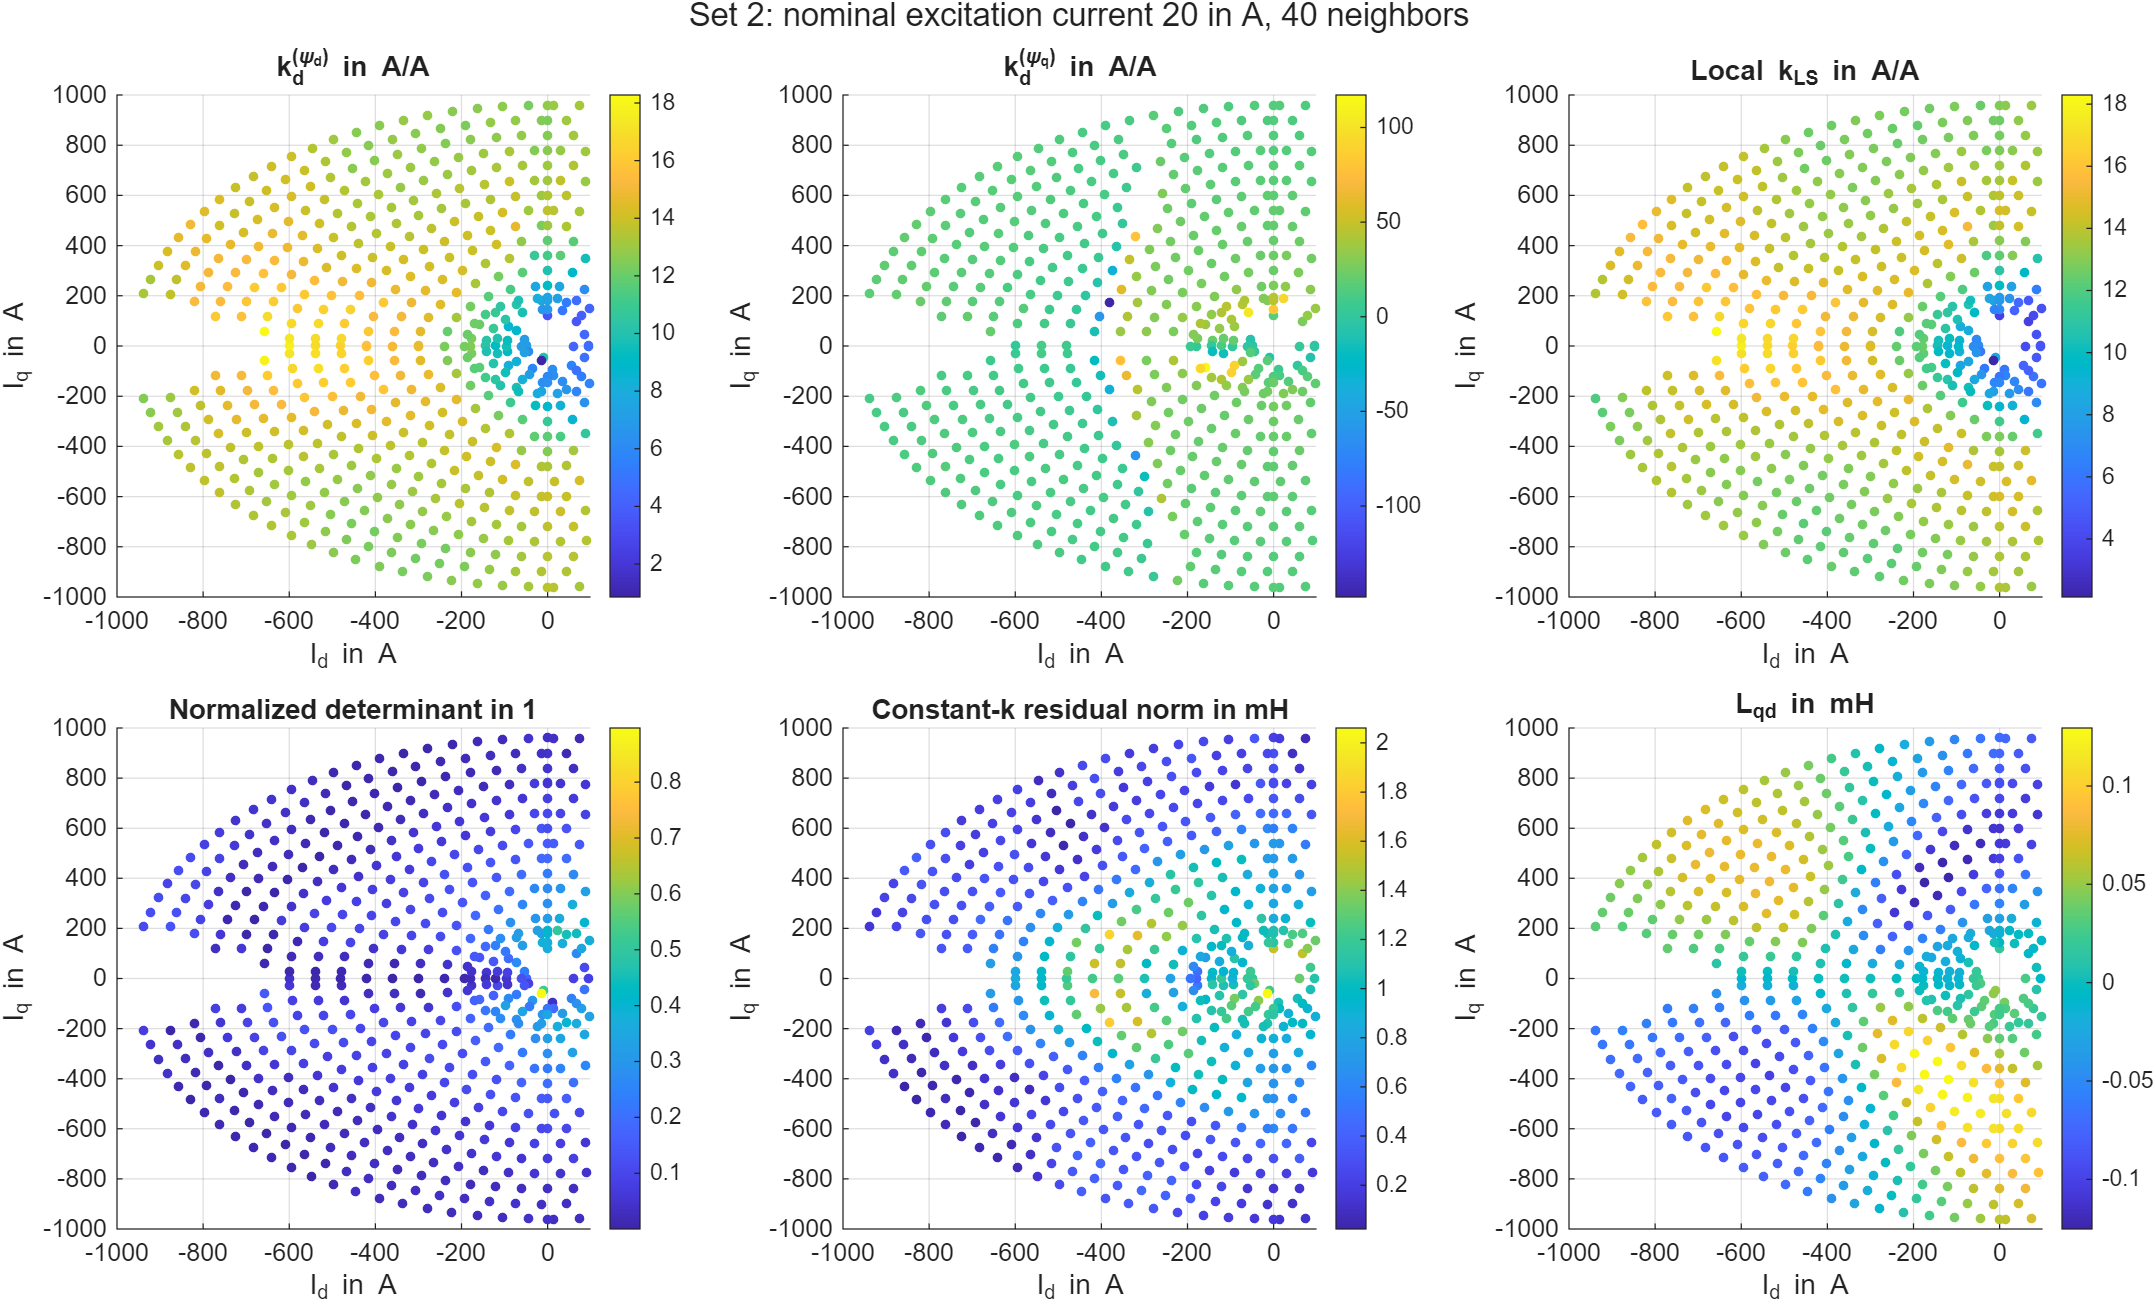
\includegraphics[width=\linewidth]{local_set2.png}
\caption{Local diagnostics for the Set 2 group with nominal excitation current 20 in A. The lower panels show normalized determinant, constant-\(k_{\mathrm{ME}}\) residual magnitude, and the cross-inductance responsible for poor conditioning of \(L_{qe}/L_{qd}\). Values use actual measured currents. Missing estimates follow the stated neighborhood and denominator rules.}
\label{fig:local}
\end{figure}

\subsection{Sensitivity to the derivative neighborhood}
\SensitivityTable
\begin{figure}[htbp]
\centering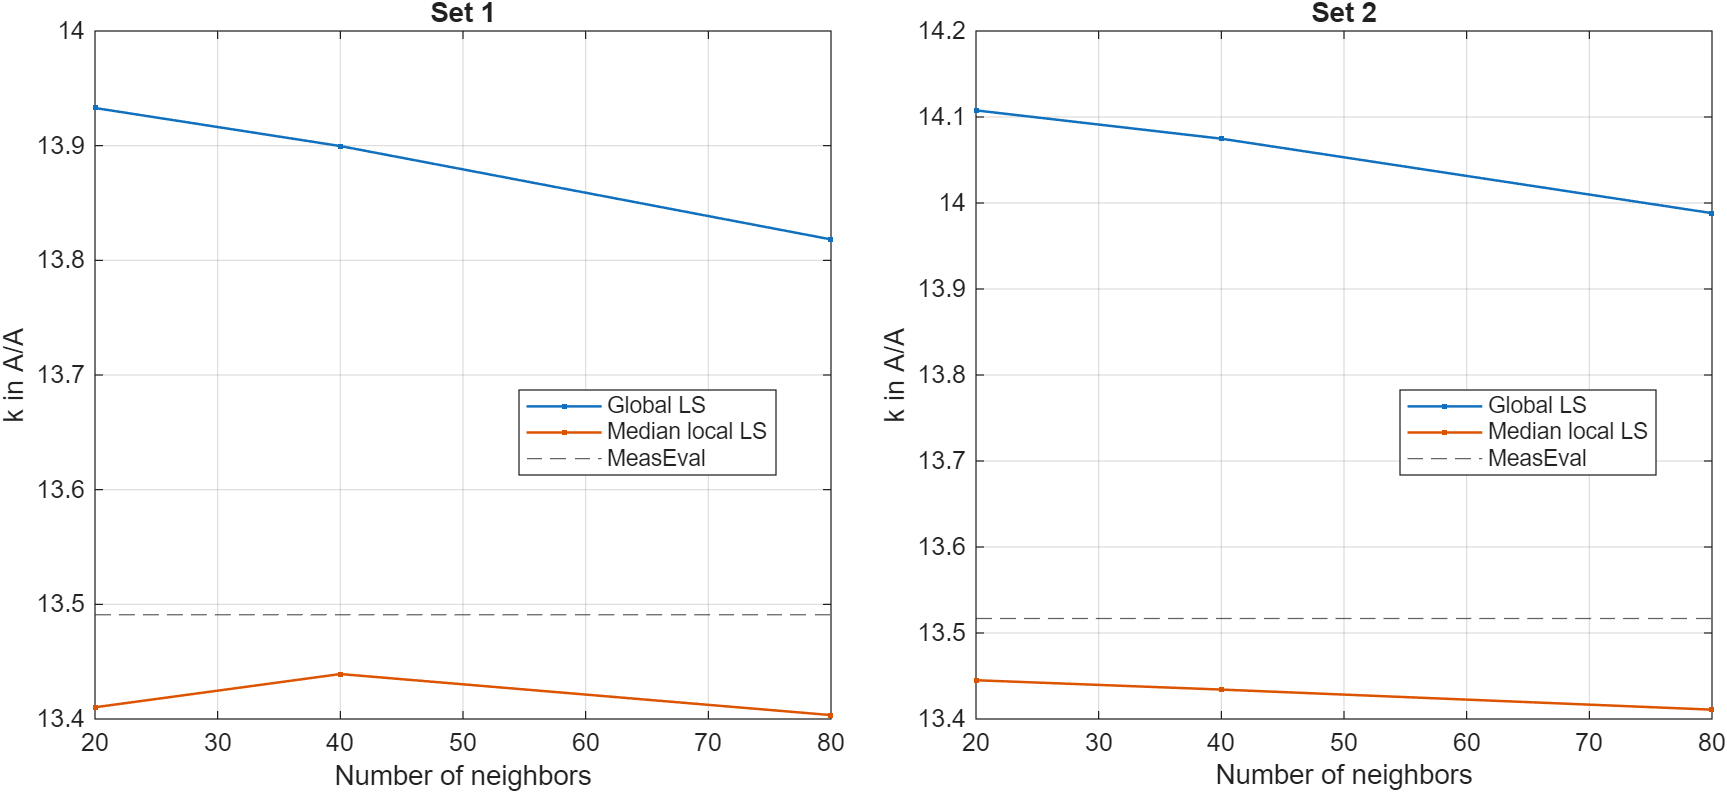
\includegraphics[width=\linewidth]{sensitivity.png}
\caption{Neighborhood sensitivity on identical retained current points within each dataset. The median local factor and global LS factor use different weighting rules.}
\end{figure}
The common-point comparison separates neighborhood-size effects from changing availability of evaluation points. The global factor remains near 14 under the investigated smoothing choices. Individual ratios and residuals remain neighborhood-dependent. This limited comparison supplies neither an optimal bandwidth nor a confidence interval for the true derivatives.

\subsection{Predicting entire missing excitation groups}
\PredictionTable
\begin{figure}[htbp]
\centering
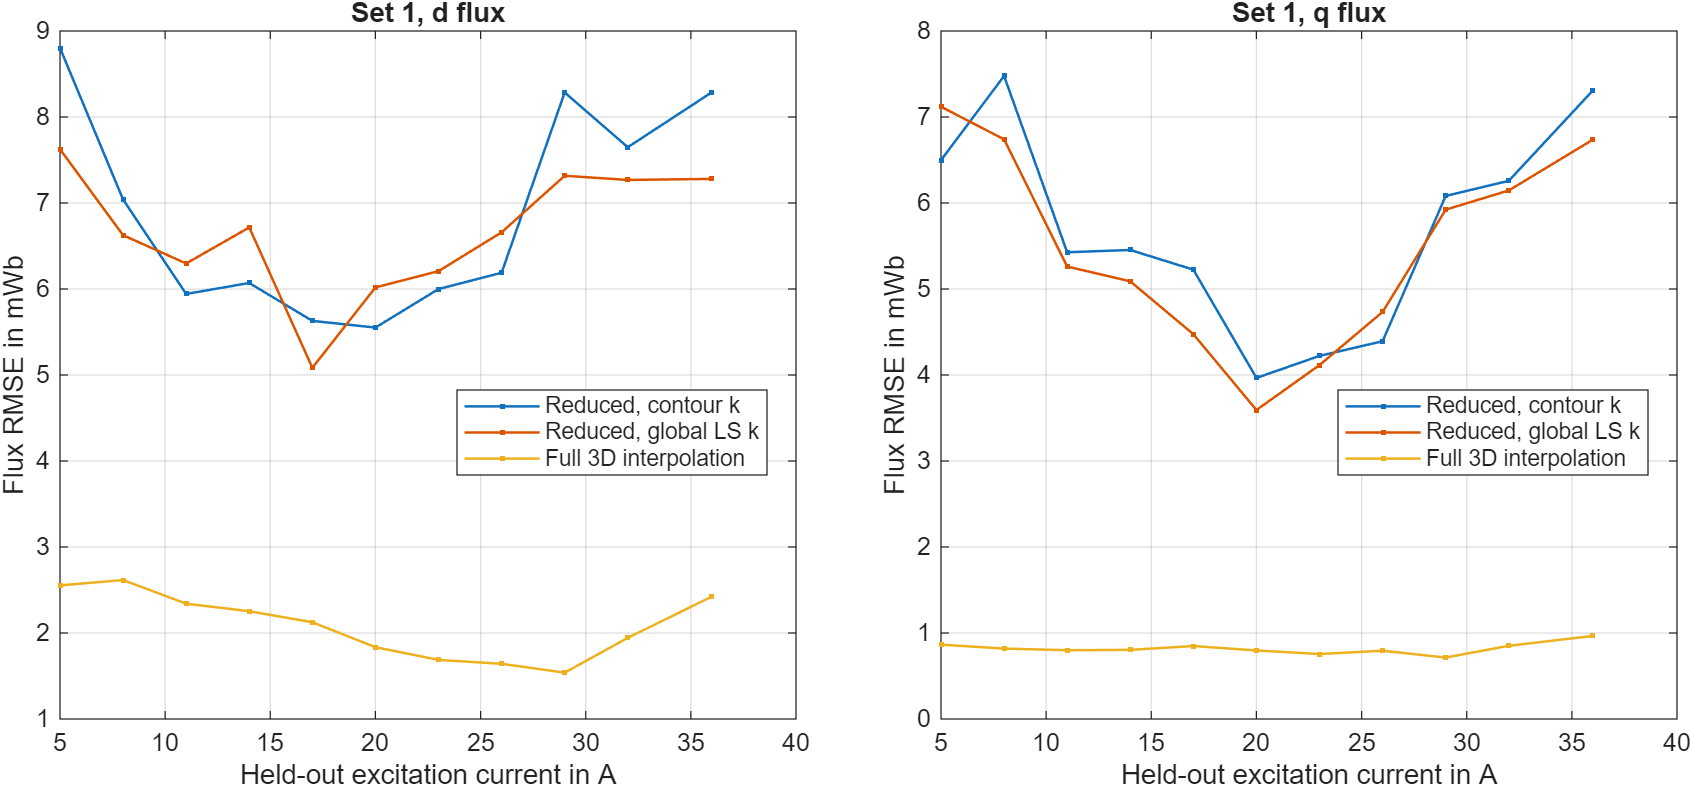
\includegraphics[width=\linewidth]{prediction_set1.png}\\[5pt]
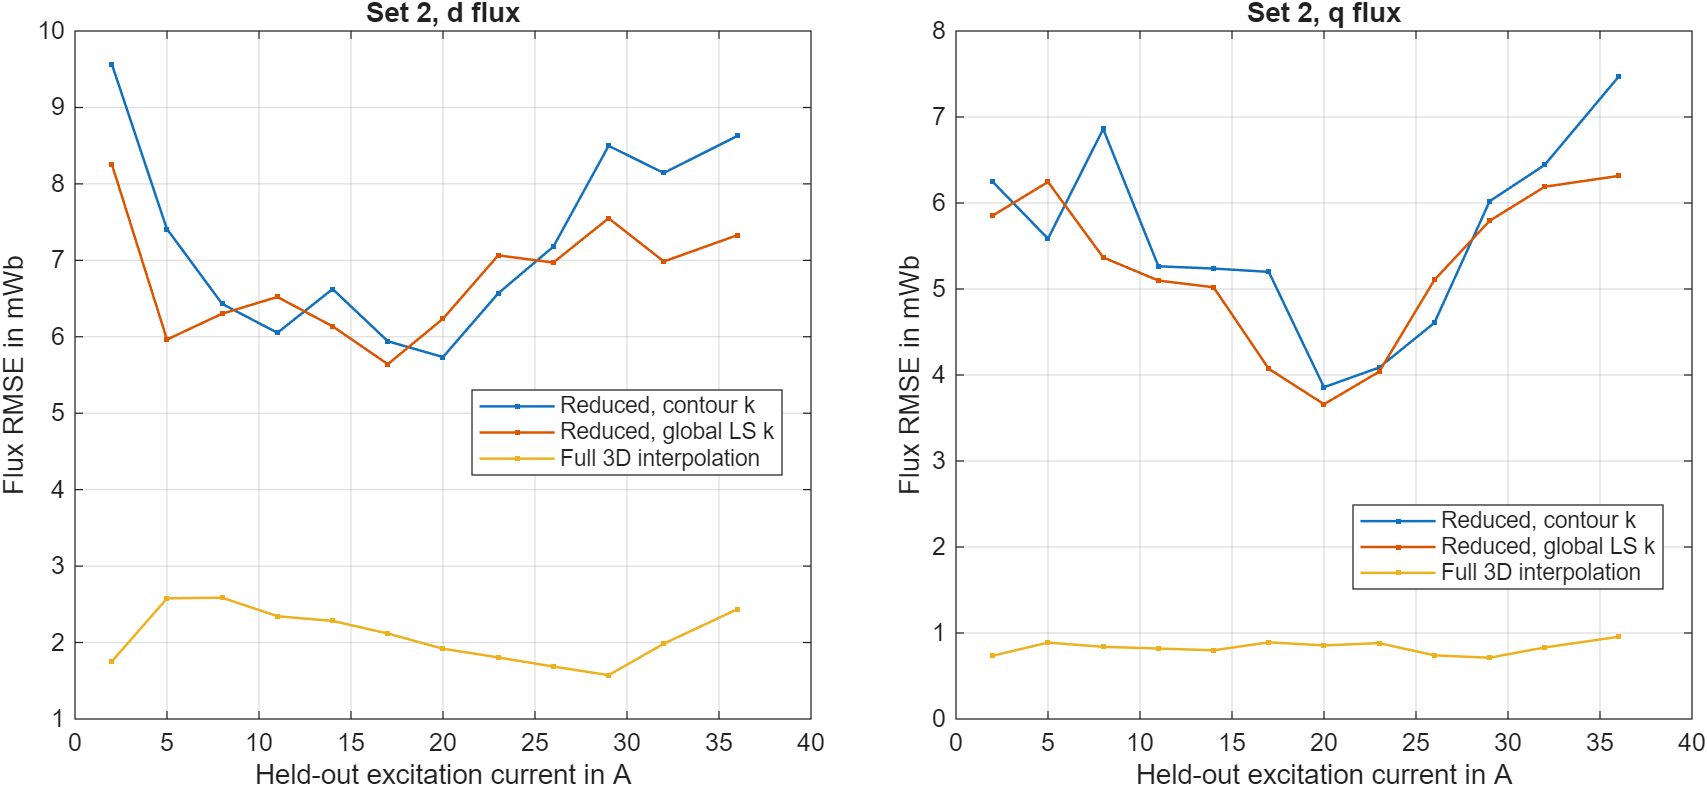
\includegraphics[width=\linewidth]{prediction_set2.png}
\caption{Per-group holdout errors on common prediction support. Each point represents a whole excitation group omitted during fitting. Both factors are recomputed without that group.}
\label{fig:prediction}
\end{figure}
Full 3D interpolation has lower aggregate d- and q-flux RMSE for both datasets. Replacing the contour factor by the global derivative factor improves the reduced predictors, but does not close the gap. Reducing a derivative residual and minimizing unseen flux error are different objectives.

The observed difference also depends on interpolation geometry, coverage, noise, and the model classes used. It does not prove that no nonlinear two-coordinate representation could work. Common support retains 6238 of 6348 interior-group points in Set 1 and 6819 of 6936 in Set 2. Boundary excitation groups are excluded by construction. Appendix~\ref{app:folds} lists the fold counts and factors.

\subsection{Added rasterization error}
\RasterTable
\begin{figure}[htbp]
\centering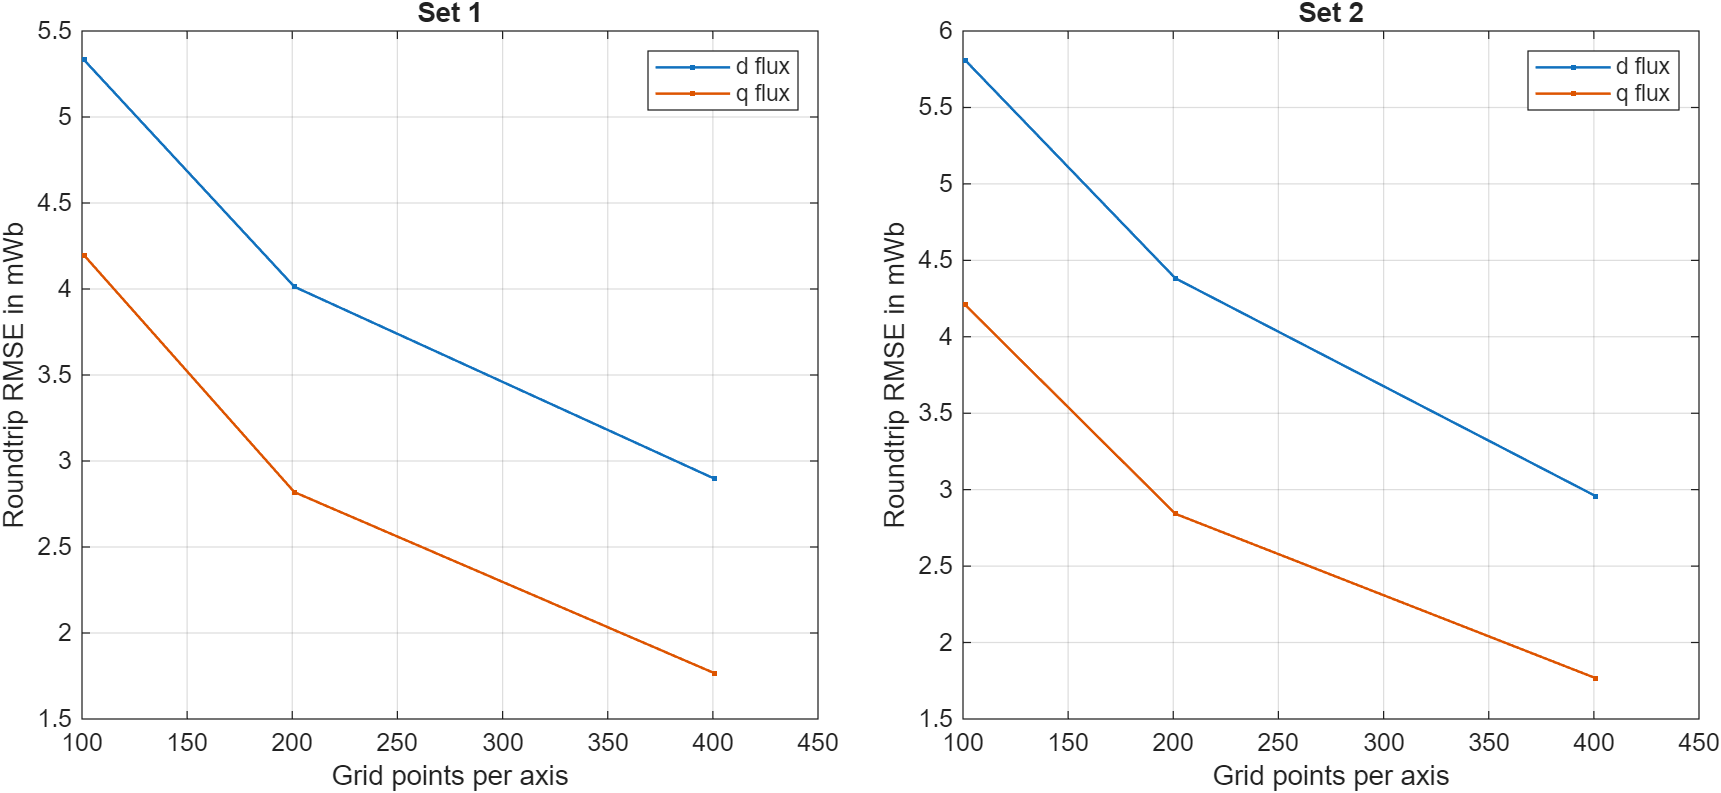
\includegraphics[width=\linewidth]{raster.png}
\caption{Bilinear roundtrip error for the same all-data reduced scattered field at three raster resolutions. Each dataset uses one common point mask across resolutions. These are reconstruction errors, not the prediction errors of Figure~\ref{fig:prediction}.}
\label{fig:raster}
\end{figure}
Increasing raster resolution reduces average return error. Substantial maximum errors remain, and individual maxima need not decrease monotonically. This establishes a processing contribution for the chosen interpolation path; it does not assign every discrepancy to an incorrect physical coordinate model.

At original scattered nodes the interpolant reproduces its training values by construction. Because all projected nodes can be distinct, that identity alone does not validate lossless 3D-to-2D reduction.

\section{Impact of Excitation-Current Coordinate Reduction on Flux-Linkage Reconstruction Accuracy}\label{sec:mapreduction}
\subsection{Question and exact reduction condition}
The processing hypothesis is that a substantial discrepancy appears when the separate excitation measurements are projected, merged, rasterized, and queried as a single two-dimensional flux map. This section compares the actual saved artifacts with their own source measurements. A reconstruction discrepancy alone does not prove a physical dimensional-reduction error.

At fixed reduced coordinates \(s=i_d+ki_e\) and \(q=i_q\), the chain rule gives
\begin{equation}\label{eq:fiberresidual}
\left.\frac{\partial\widehat{\ps}}{\partial i_e}\right|_{s,q}
=\begin{bmatrix}L_{de}\\L_{qe}\end{bmatrix}
-k\begin{bmatrix}L_{dd}\\L_{qd}\end{bmatrix}
=\bvec-k\avec.
\end{equation}
Along any admissible connected constant-\((s,q)\) section,
\begin{equation}
\ps(s-ke_2,q,e_2)-\ps(s-ke_1,q,e_1)
=\int_{e_1}^{e_2}(\bvec-k\avec)(s-ke,q,e)\,\dd e.
\end{equation}
Thus the reduction preserves all stator-flux information under the conditions established in Section~\ref{sec:common}: both coupling equations must hold, together with the domain connectivity requirement. A violation at a point prevents an exact reduction in its neighborhood for that constant \(k\). The derivative estimates are numerical diagnostics of this condition, not exact measurements of its violation.

The pure coordinate shear leaves each source flux value unchanged. If two physical points have identical reduced coordinates but different fluxes, no single-valued reduced function can reproduce both. Here all projected measured coordinates are distinct: 7476 of 7476 in Set 1 and 8092 of 8092 in Set 2. Consequently, exact source-node interpolation is possible even for a physically unsuitable reduction. The triangulation may then represent incompatible slices through strong variations between nearby nodes.

\subsection{Saved representations and coordinate conventions}
The standalone script \texttt{analyze\_flux\_map\_reduction.m} loads the original local FluxEval files and evaluates:
\begin{itemize}
\item A: \texttt{Meas.PE\_psi\_d\_meas} and \texttt{PE\_psi\_q\_meas} at actual measured \((i_d,i_q,i_e)\).
\item B: \texttt{LUT.CtrlMaps.complete}, retaining separate source excitation-reference slices.
\item C: \texttt{LUT.CtrlMaps}, queried at measured \((i_d+ki_e,i_q)\), using its saved \texttt{EESM\_winding\_ratio}.
\end{itemize}
The saved factors are \(13.490937385\) for Set 1 and \(13.516845982\) for Set 2. Each slice is associated with its matching \texttt{complete.I\_exc\_vec} value, rather than an assumed field or array order.

The saved \texttt{complete} files have no coordinate metadata, and their d breakpoints coincide with the corresponding physical \texttt{Calc.Grid.Id\_fine} axes. The script queries them with measured physical \(i_d\). Newer local \texttt{Torque\_LUT\_Calc.m} source also supports relabelled complete slices with
\[
d_{\mathrm{slice}}^*=i_d+k_{\mathrm{slice}}I_{e,\mathrm{ref}}.
\]
For those slices, the documented \texttt{Coordinates.d\_axis} is used and the query receives the fixed slice-reference offset. Substituting pointwise measured \(i_e\) into that relabelling would change the physical lookup location within the already constructed slice. The merged map, in contrast, is built from pointwise measured excitation currents and requires those same measured currents at lookup.

Both B and C are queried with bilinear \texttt{interp2}. Out-of-domain or NaN-contaminated interpolation cells remain invalid; no extrapolation or zero filling is used. This specifies the diagnostic lookup operator, not the operator of every GUI or controller consumer. Nominal excitation values only assign groups. Requested stator currents are never substituted for measured query coordinates.

B is a collection of separate two-dimensional representations of the recorded groups, not a continuously interpolated three-current model. Small excitation-current fluctuations within each group remain present in its source data. Only the 3000 rpm group is available in the two selected full evaluations, so no comparison across machine speeds is possible here.

\subsection{Residuals, coverage, and saved-map comparison}
For \(x\in\{d,q\}\), define
\[
r_{x,B}=\psi_{x,B}-\psi_{x,A},\qquad r_{x,C}=\psi_{x,C}-\psi_{x,A}.
\]
A method's own mask requires both returned flux components to be finite. The common mask is the intersection of these masks. RMSE and maximum absolute residual are calculated componentwise on the stated mask. Figures comparing B with C use the common mask; the MAT output retains both masks, both summaries, and per-excitation summaries.

\begin{table}[htbp]
\centering\small
\caption{Saved-map reconstruction errors, all in mWb. Own support is method-specific; common support uses identical points for B and C within each dataset. Source counts are 7476 and 8092.}\label{tab:savedmaps}
\begin{tabular}{cllrrrrr}
\toprule
Set & Map & Mask & \(N\) & RMSE d & RMSE q & Max d & Max q\\
\midrule
1 & B: complete & Own & 6761 & 0.292 & 0.178 & 7.503 & 1.870\\
1 & C: merged & Own & 7357 & 5.336 & 4.169 & 38.497 & 28.765\\
1 & B: complete & Common & 6759 & 0.292 & 0.178 & 7.503 & 1.870\\
1 & C: merged & Common & 6759 & 5.538 & 4.331 & 38.497 & 28.765\\
\midrule
2 & B: complete & Own & 7319 & 0.313 & 0.177 & 7.392 & 1.792\\
2 & C: merged & Own & 7968 & 5.665 & 4.173 & 44.725 & 29.880\\
2 & B: complete & Common & 7315 & 0.313 & 0.174 & 7.392 & 1.751\\
2 & C: merged & Common & 7315 & 5.884 & 4.333 & 44.725 & 29.880\\
\bottomrule
\end{tabular}
\end{table}

The complete slices reproduce their source measurements much more closely on average than the merged map. Their maxima show that even B is not exact. Its residual includes the existing individual map construction and the bilinear return; the separate excitation maps have already been resampled.

Figures~\ref{fig:savedset1} and~\ref{fig:savedset2} show both components against source values, physical current-space residuals, and RMSE by excitation reference. In Set 2 the merged d-flux RMSE ranges from approximately \(3.85\) to \(8.12\) mWb across groups. The q-flux RMSE is approximately \(1.99\) mWb at 20 A and \(7.25\) mWb at 40 A. Set 1 shows a similar increase towards high excitation. Thus the discrepancy is structured in current space and excitation, rather than a single constant flux offset.

\begin{figure}[p]
\centering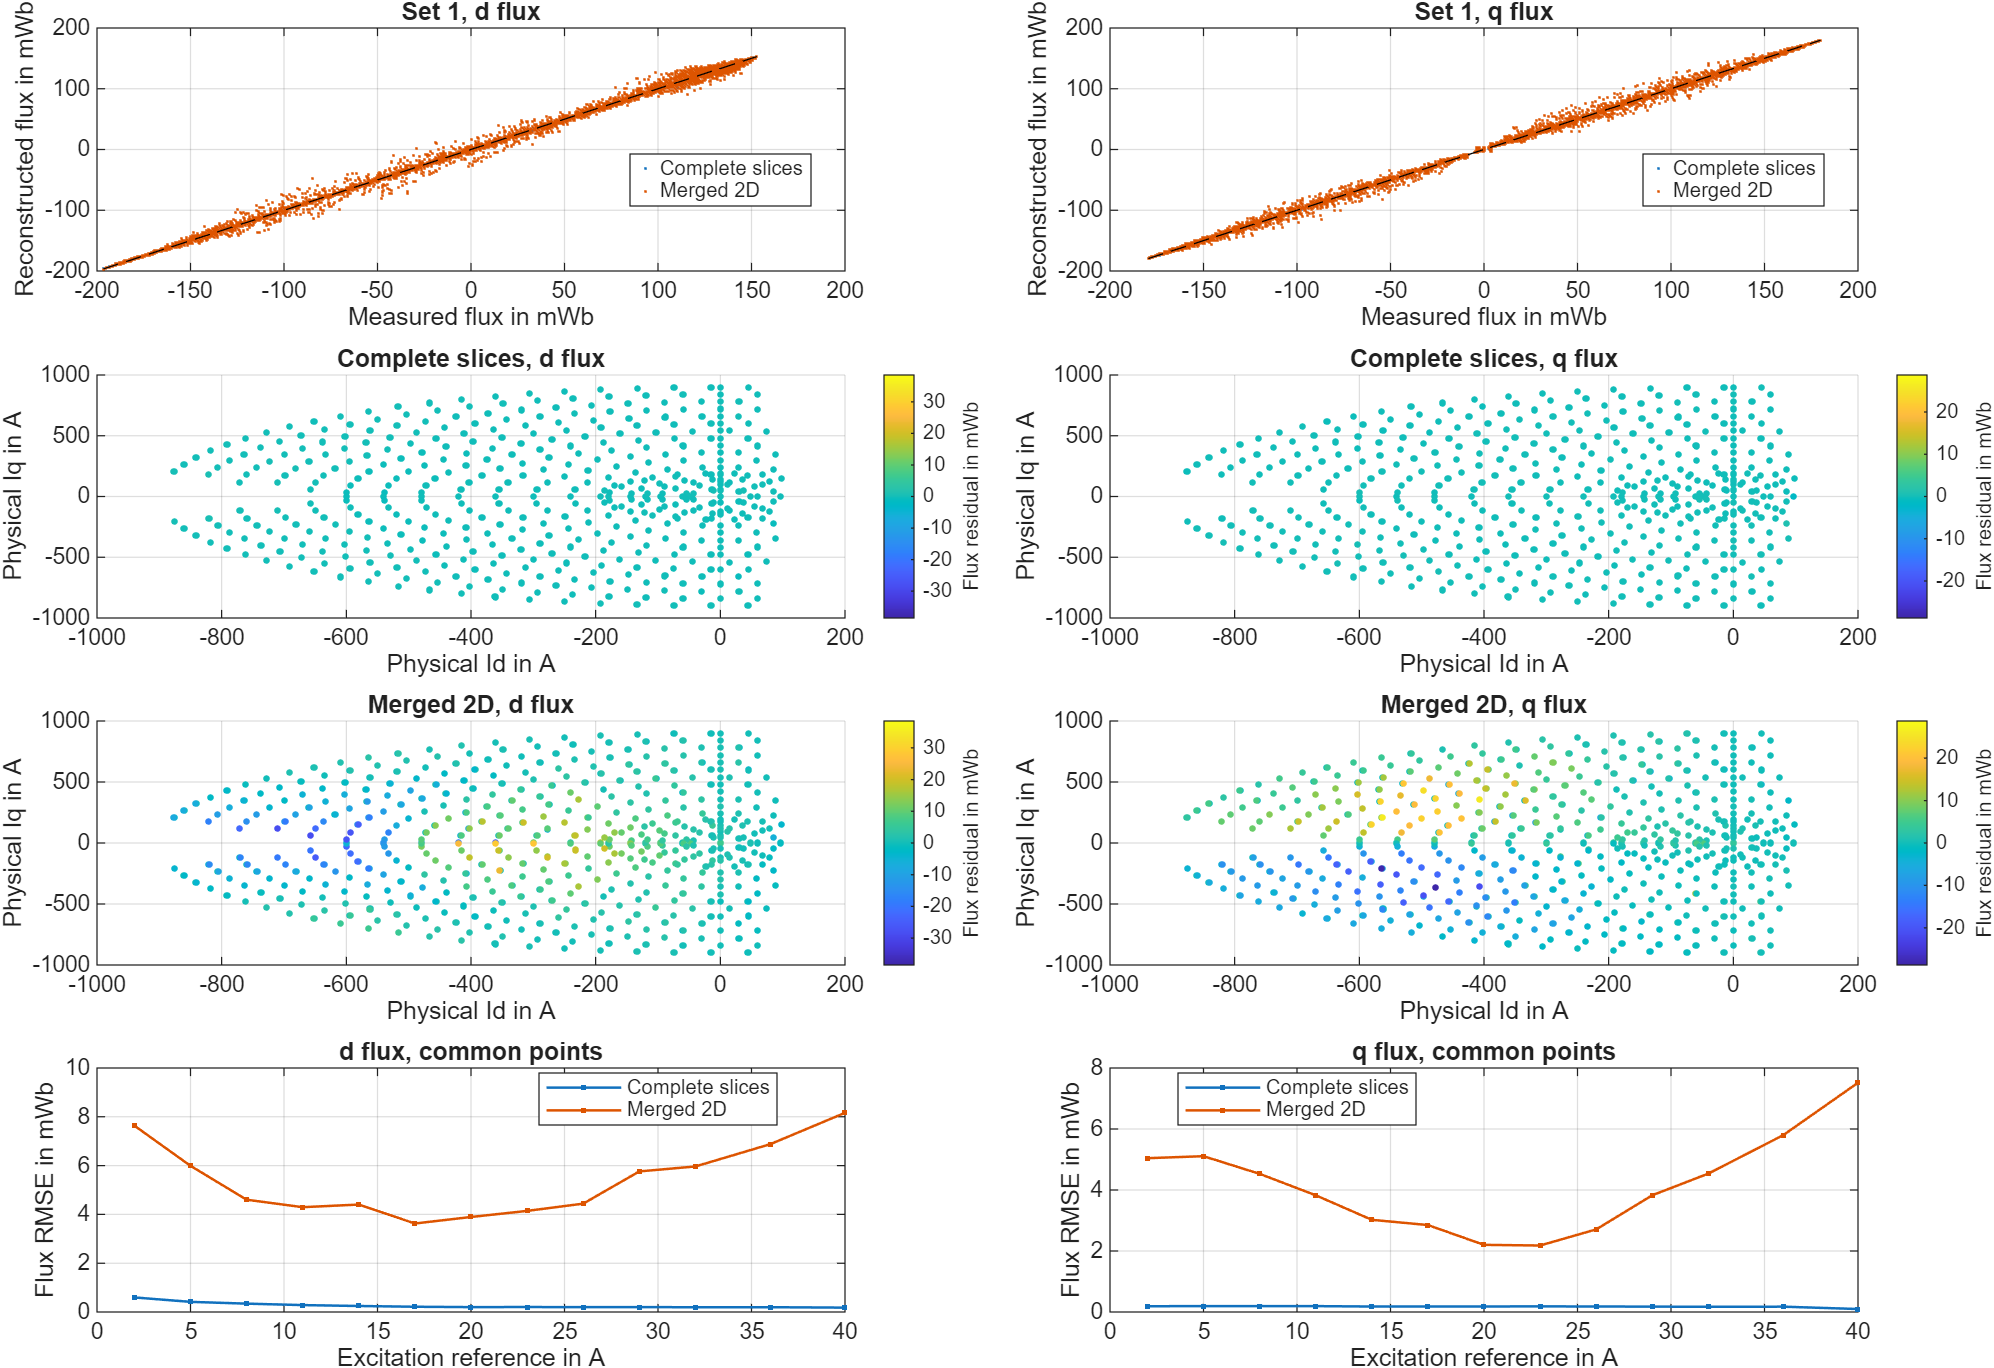
\includegraphics[width=\linewidth,height=0.84\textheight,keepaspectratio]{reduction_set1.png}
\caption{Set 1 on 6759 common points. Rows: reconstructed versus measured flux, complete-slice residuals, merged-map residuals, and per-group RMSE. Residuals are returned minus measured. Within each flux component the spatial panels share color limits. Spatial plots overlay excitation groups; bottom panels retain group distinctions.}\label{fig:savedset1}
\end{figure}
\begin{figure}[p]
\centering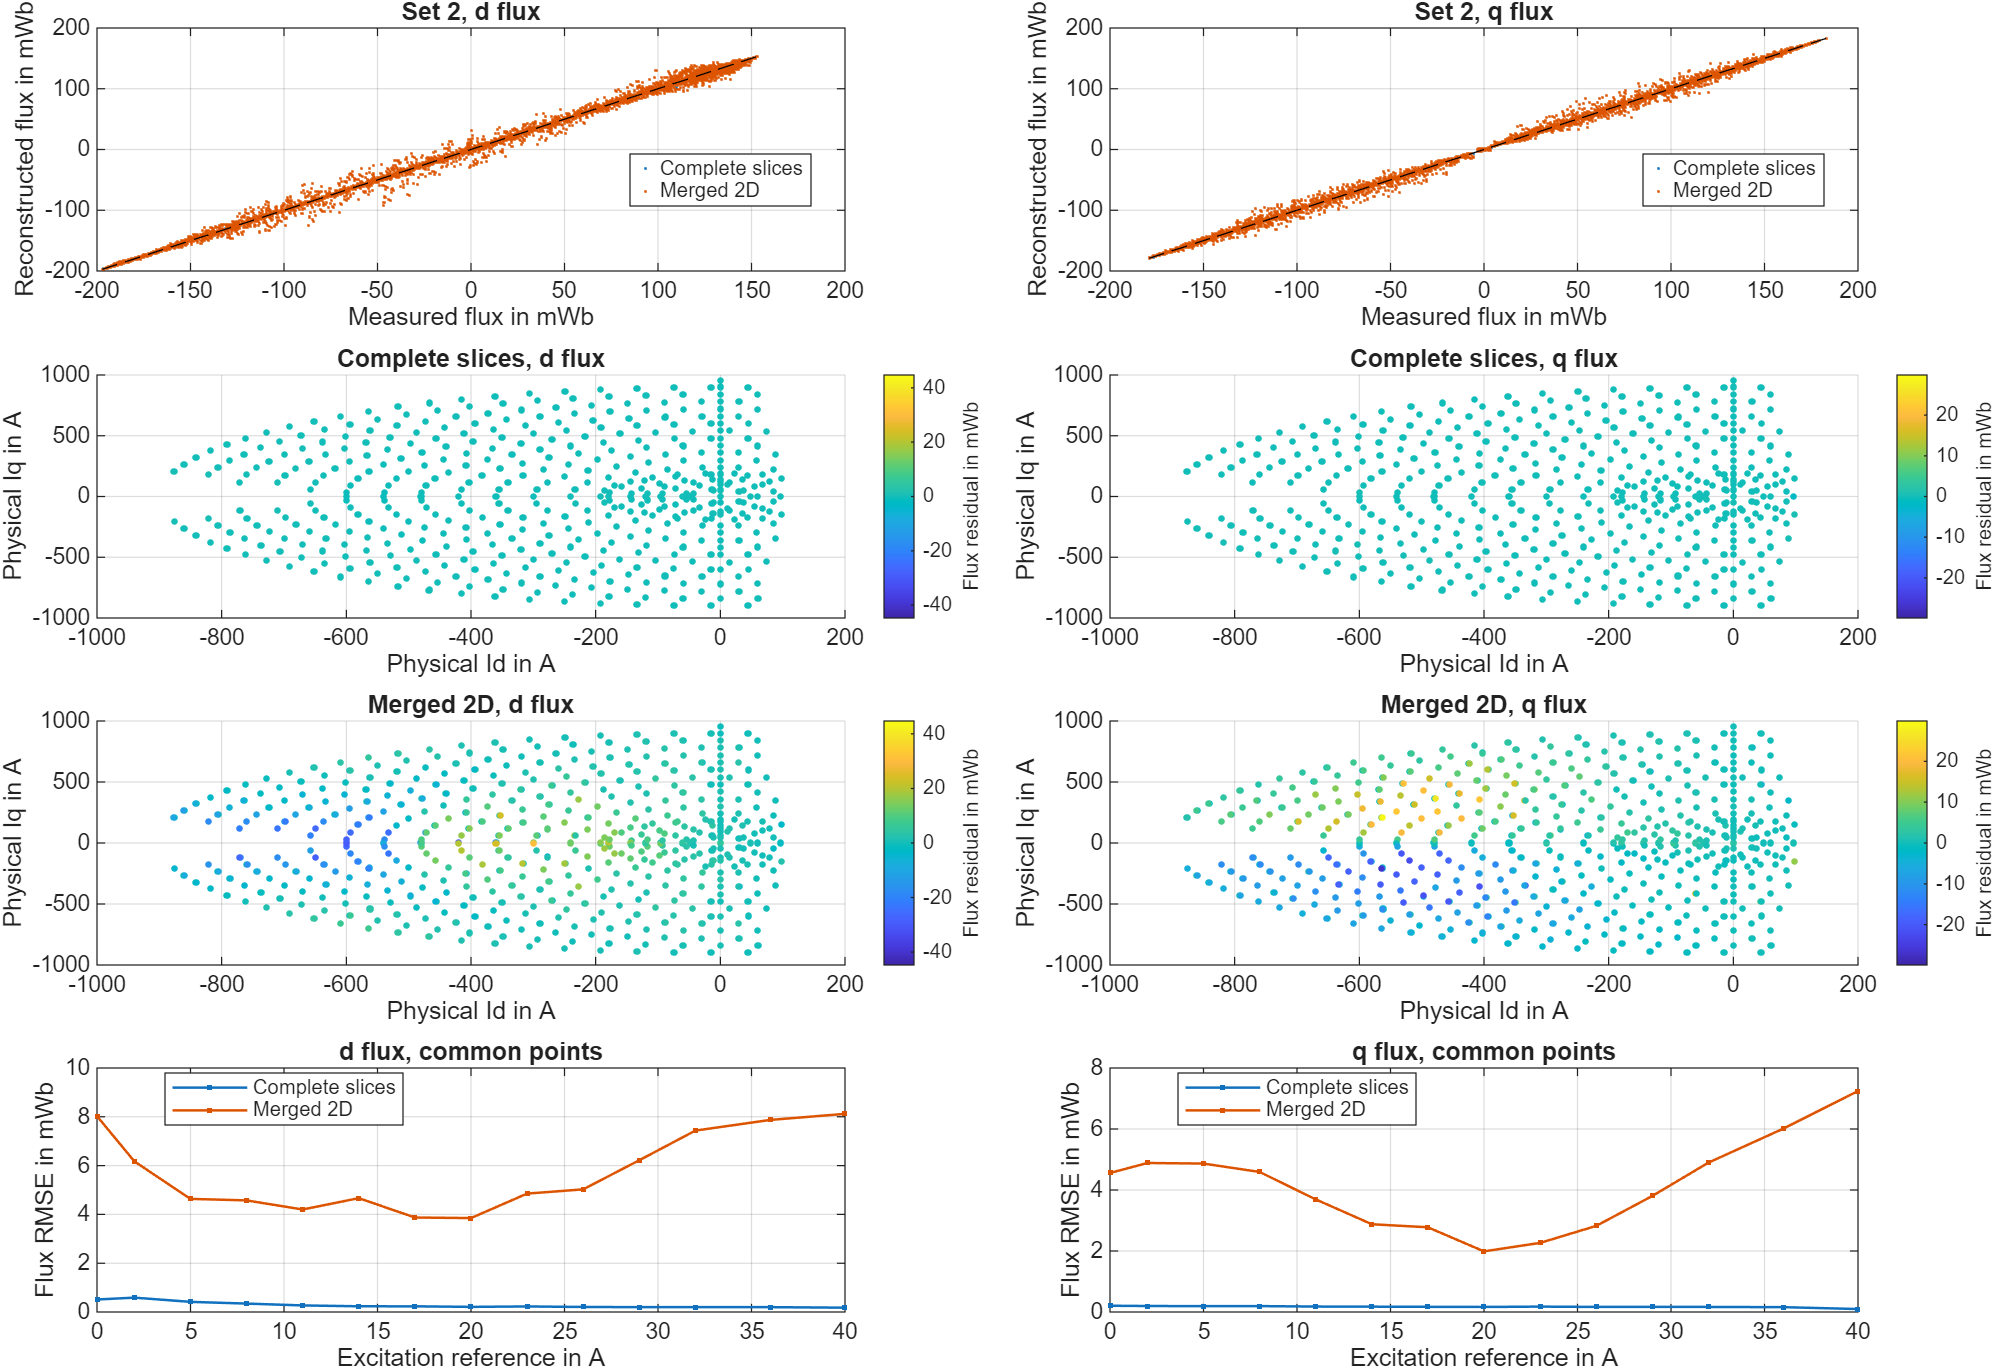
\includegraphics[width=\linewidth,height=0.84\textheight,keepaspectratio]{reduction_set2.png}
\caption{Set 2 on 7315 common points. Complete-slice residuals are close to zero on the color scale required for the merged residuals. Each group uses its own common-point subset: the bottom panels do not imply identical physical current support across excitation references.}\label{fig:savedset2}
\end{figure}

\subsection{Separating source arithmetic, gridding, and model reduction}
Using stored averaged measured voltages, measured stator currents, stored \(R_s\), and averaged electrical angular speed, the stationary formulas reproduce A to a maximum absolute discrepancy below \(1.4\,10^{-17}\) Wb. This establishes arithmetic consistency with the saved processed signals. It cannot establish their absolute calibration or rule out errors inherited from measurement and preprocessing.

The saved map branches are parallel. Complete slices originate in individual \texttt{Calc.Grid} representations, whereas the merged flux grid is constructed directly from sheared measured flux samples. B is not an intermediate stage through which C necessarily passes. Subtracting their RMSE values, or assigning the squared-error difference to one independent physical cause, would be unjustified.

Rebuilding the saved merged grid from measured projected points with linear scattered interpolation reproduces its finite flux values to roundoff. The scattered field also reproduces original source nodes to roundoff. The nonzero C--A residual therefore appears when that same scattered field is sampled onto the saved regular grid and bilinearly returned to source coordinates. This gives a direct operational explanation of the observed saved-map return error without requiring a new flux calculation or a changed machine speed.

To quantify this operation, keep the saved factor, saved axis extents, and underlying scattered field fixed, and vary only regular-grid size. These extents differ from the measured-coordinate bounds of the earlier controlled experiment in Section~\ref{sec:numerics}. Use one common finite mask across resolutions, restricted to original merged-map support.

\begin{table}[htbp]
\centering\small
\caption{Raster roundtrip on saved axis extents and fixed masks. Errors are in mWb. The 101-node row reproduces the saved map's own-support result.}\label{tab:savedraster}
\begin{tabular}{crrrrrr}
\toprule
Set & Nodes per axis & \(N\) & RMSE d & RMSE q & Max d & Max q\\
\midrule
1 & 101 & 7357 & 5.336 & 4.169 & 38.497 & 28.765\\
1 & 201 & 7357 & 3.991 & 2.809 & 39.696 & 29.679\\
1 & 401 & 7357 & 2.721 & 1.779 & 40.154 & 24.578\\
2 & 101 & 7968 & 5.665 & 4.173 & 44.725 & 29.880\\
2 & 201 & 7968 & 4.235 & 2.810 & 43.216 & 29.419\\
2 & 401 & 7968 & 2.977 & 1.742 & 42.143 & 23.468\\
\bottomrule
\end{tabular}
\end{table}

Average errors decrease substantially with resolution, but large maxima remain and need not decrease monotonically. This is consistent with steep local variations in the merged scattered field; it does not demonstrate that every such variation arises from invalid physical reduction. Exact source-node return is also not evidence of lossless reduction: interpolation has seen every source value. The missing-excitation-group experiment in Section~\ref{sec:holdout} supplies the complementary prediction check.

\subsection{A small constant-factor variation}
The script repeats the merged construction for \(k=12,12.5,\ldots,16\), additionally including each saved factor. Saved \(101\times101\) axis coordinates remain fixed. Each candidate changes projected measured points, triangulation, and query positions, while retaining source flux values. A single mask is used for every candidate and both components, also restricted to B--C common support: 6658 points in Set 1 and 7196 in Set 2.

The best sampled candidate minimizes \(\operatorname{RMSE}_d^2+\operatorname{RMSE}_q^2\). All measured samples also train these fields. This is a reconstruction diagnostic, not predictive factor selection; intermediate candidate values have not been optimized.

\begin{table}[htbp]
\centering\small
\caption{Saved and best sampled factors on fixed sweep masks. Errors are in mWb; \(k\) is in A/A. These masks differ from Table~\ref{tab:savedmaps}.}\label{tab:ksweep}
\begin{tabular}{clrrrrrr}
\toprule
Set & Candidate & \(k\) & \(N\) & RMSE d & RMSE q & Max d & Max q\\
\midrule
1 & Saved & 13.49094 & 6658 & 5.575 & 4.362 & 38.497 & 28.765\\
1 & Best sampled & 14.00000 & 6658 & 4.879 & 4.120 & 32.135 & 28.142\\
2 & Saved & 13.51685 & 7196 & 5.928 & 4.368 & 44.725 & 29.880\\
2 & Best sampled & 14.50000 & 7196 & 5.067 & 4.043 & 31.094 & 25.916\\
\bottomrule
\end{tabular}
\end{table}

The combined RMS magnitude decreases by approximately 9.8 percent in Set 1 and 12.0 percent in Set 2. Neither candidate approaches the average accuracy of the separate saved slices. The d and q components prefer different trends as \(k\) changes, consistent with satisfying two flux constraints together. The best sampled reconstruction factor need not equal the derivative-based global factor: objectives and interpolation effects differ.

\begin{figure}[htbp]
\centering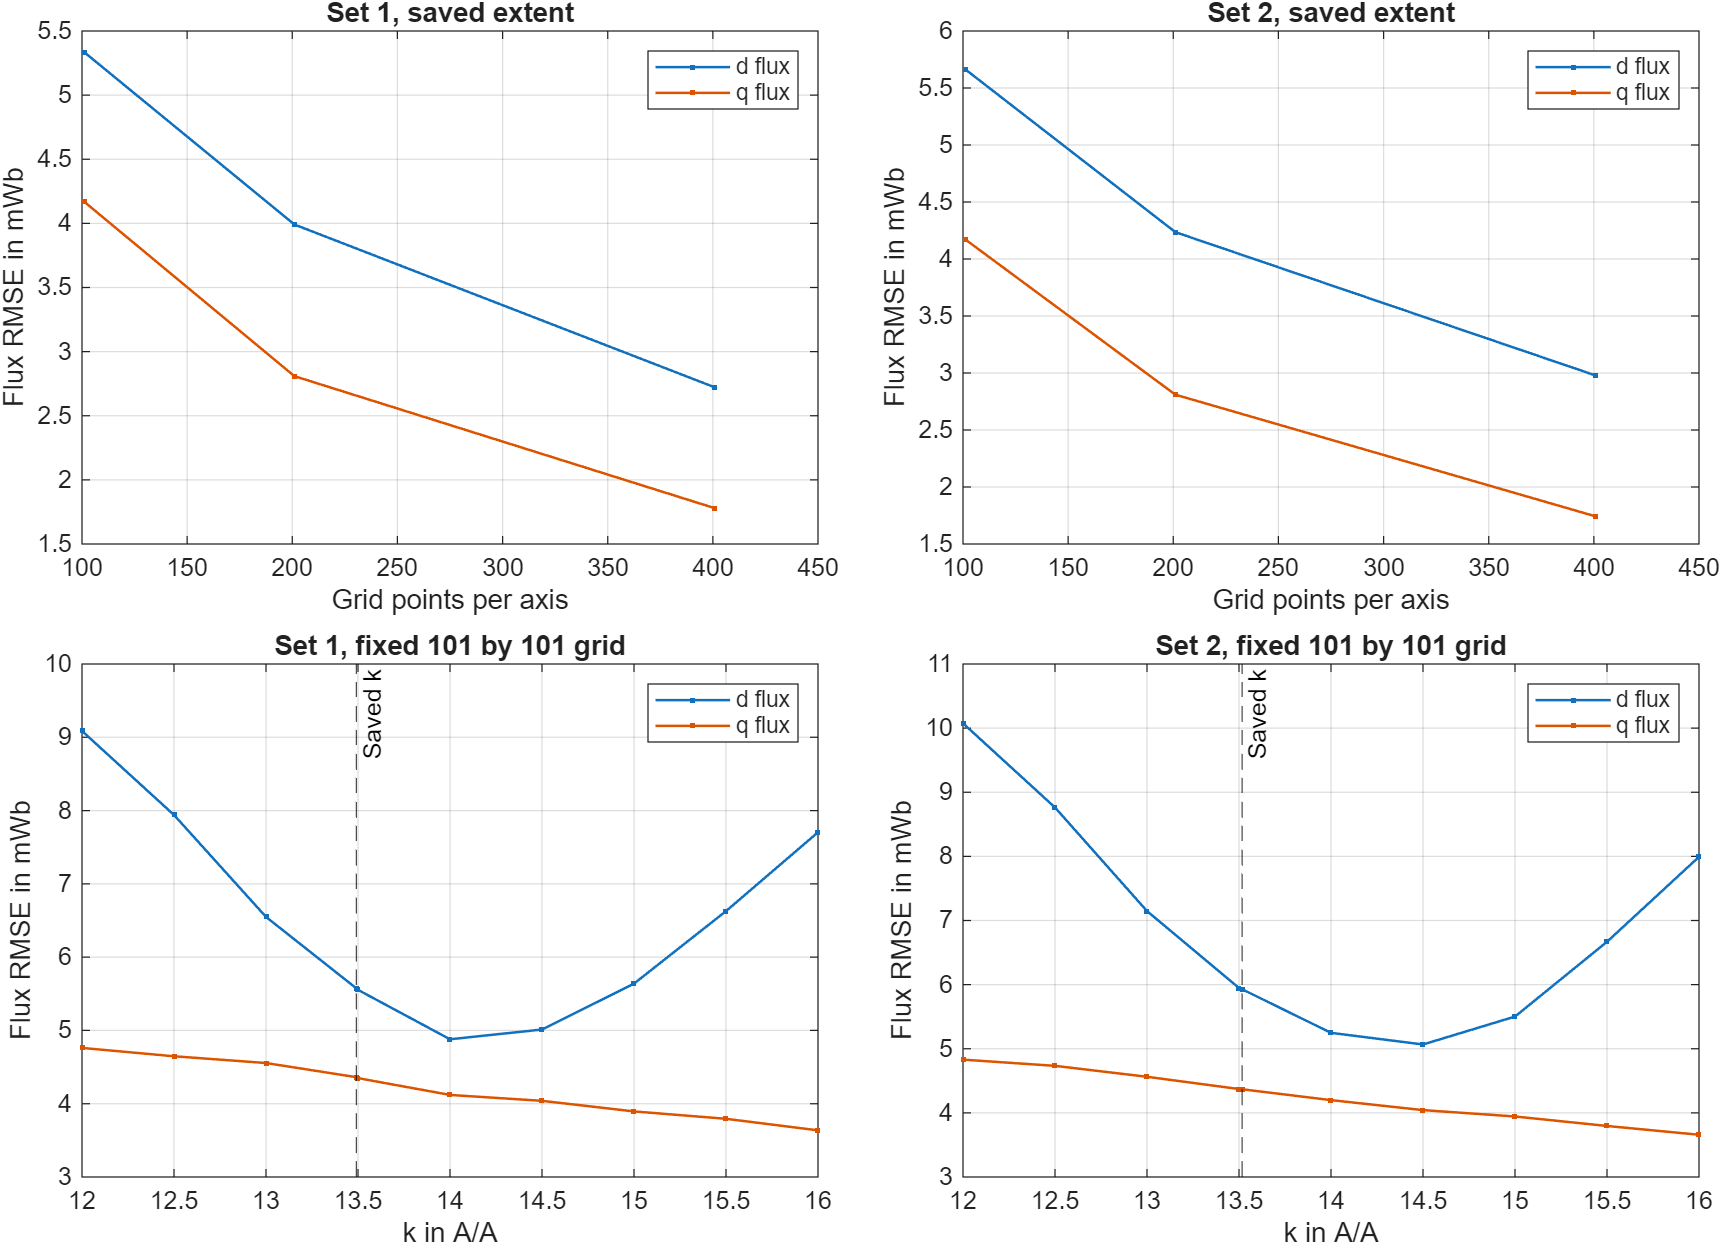
\includegraphics[width=\linewidth]{reduction_processing.png}
\caption{Saved-extent raster refinement at fixed saved \(k\) (top) and the small \(k\) sweep at fixed raster axes (bottom). Masks are fixed within each comparison but differ between top and bottom. Dashed lines mark saved factors.}\label{fig:reductionprocessing}
\end{figure}

\subsection{Established findings and consequence for MeasEval}
\begin{enumerate}
\item The coordinate shift itself changes no flux value. The stationary calculation is consistent with stored inputs to roundoff; absolute measurement accuracy remains unresolved.
\item Individual slice construction and lookup introduce small average residuals, with some larger isolated errors.
\item The actual merged-grid roundtrip creates much larger reconstruction residuals. Refinement demonstrably reduces their average magnitude. This identifies an interpolation and representation effect at the original measurement speed.
\item Changing one constant factor improves the tested result moderately but does not remove its discrepancy. This sweep cannot assign a numerical percentage to physical information loss: it also changes triangulation and raster sampling.
\item The separate derivative and whole-group holdout results provide additional evidence against an exact common constant reduction over this domain. The tested three-current predictor has lower missing-group errors. A complete causal partition of measurement noise, interpolation, and structural reduction error is not identified.
\end{enumerate}
A full three-current representation retains excitation explicitly and avoids imposing equation~\eqref{eq:fiberresidual} as zero. It still needs adequate sampling, suitable interpolation, and reliable measurements; it is not automatically exact. The evidence favors investigating it when accuracy across excitation is required. Improving the constant factor and raster resolution remain useful approximations, but their benefit should be checked with withheld excitation groups rather than source-node reconstruction alone.



\section{Physical interpretation and implications for MeasEval}\label{sec:physical}
\subsection{Coordinate replacement preserves source flux values}
The transformation
\[
(i_d,i_q,i_e,\psi_d,\psi_q)\mapsto(i_d+k_0i_e,i_q,\psi_d,\psi_q)
\]
leaves both flux values unchanged. Changing flux values requires a subsequent interpolation, averaging, or approximation. Appendix~\ref{app:existing} visualizes this distinction.

The results support \(k_{\mathrm{ME}}\) as a practical summary over its selected contour range. They do not justify identifying it with an exact geometric turns ratio, every local derivative ratio, or an everywhere-valid common constant reduction. Omitting the lowest and highest flux quarters during factor estimation matters when applying that factor at those extremes.

\subsection{A flux table does not establish complete PSM equivalence}
Even if~\eqref{eq:reduced} were exact, the physical currents remain \(i_d=s-k_0i_e\), \(i_q=q\). For the amplitude-invariant dq convention, the torque identity becomes
\begin{align}
T_e&=\tfrac32p(\psi_d i_q-\psi_q i_d)\\
&=\tfrac32p\bigl[f(s,q)q-g(s,q)s+k_0i_e g(s,q)\bigr].
\end{align}
An explicit excitation term remains. Substituting \(s\) directly for physical \(i_d\) in a PSM torque formula would discard it. Likewise, the d-axis resistive voltage term is \(R_s(s-k_0i_e)\), not \(R_s s\). For constant \(k_0\),
\[
\dot\psi_x=f_{x,s}(\dot i_d+k_0\dot i_e)+f_{x,q}\dot i_q,
\]
where \(f_d=f,f_q=g\). The excitation circuit retains its own voltage equation. A common two-axis flux representation does not, on its own, validate identical controller dynamics or a complete two-current machine model.

For a variable expression \(s=i_d+i_e k(\ii)\), the complete chain rule is
\[
\dot s=(1+i_e k_{i_d})\dot i_d+i_e k_{i_q}\dot i_q
+(k+i_e k_{i_e})\dot i_e.
\]
These additional terms cannot be omitted in dynamic calculations.

\subsection{Practical consequences}
Keep the original contour estimate as a named reference, preserve excitation ordering, and retain measured physical currents. Compare both stator flux constraints before interpreting a factor as a common compensation direction. Use joint residuals and denominator information alongside ratio plots.

Distinguish source flux values, a scattered merged field, a raster, and a consumer's returned values. Invalid interpolation values must remain distinguishable from measured zero flux. The controlled raster experiment here does not prescribe a replacement for the GUI or controller lookup operator.

\section{Limitations and conclusion}
These are processed GUI outputs at one requested speed. The study does not establish absolute flux calibration or quantify sensor uncertainty. It does not isolate temperature, timing, resistance, loss, or averaging effects. Whole-group holdout avoids fitting to the missing group, but records from the same campaign are not independent calibrated experiments.

Local affine derivatives trade resolution against noise and curvature bias. Missing neighborhoods, denominator thresholds, and current-space sampling affect numerical summaries. A nonzero estimated residual is not itself a statistical significance statement.

Mathematically, the common constant shift requires both equations~\eqref{eq:common}. The determinant identifies a common local direction only under the stated nondegeneracy conditions. A varying local factor does not automatically yield expression~\eqref{eq:shift}.

Numerically, the reproduced MeasEval factors are approximately 13.5. Joint derivative fitting produces global factors near 14, with coupling residuals not removed by that change. The tested full three-current interpolant predicts missing excitation groups more accurately than the constant-factor reductions. Rasterization adds a separate measurable error.

The saved-artifact diagnosis additionally locates a substantial reconstruction discrepancy in the merged-grid roundtrip. Separate saved excitation slices have much smaller average residuals. Finer rasters reduce this reconstruction error considerably, while the small constant-factor sweep gives only a moderate further improvement. These findings do not identify a unique physical cause or a quantitative partition of structural and interpolation errors.

Together these findings support an approximate, domain-dependent use of the constant factor. They motivate a three-current representation or an explicitly constructed variable coordinate only after checking local compatibility and conditioning. No such variable coordinate is claimed to have been identified here.

\appendix
\section{Source files, execution, and notation mapping}
The supplied \emph{Motor Model.note} contains three handwritten pages, read from its stored vector strokes. Page 1 supplies the voltage convention. The coordinate derivation and determinant argument on page 3 are developed in Sections~\ref{sec:contours}--\ref{sec:variable}. The full flux-differential notation on pages 2 and 3 is retained, while identification is restricted to the two measured stator functions.

The original \texttt{analyze\_winding\_factors.m} remains the finite-contour reference. Its \texttt{kd\_psid}, \texttt{kd\_psiq} are the two d-shift candidates; \texttt{kq\_psid}, \texttt{kq\_psiq} are the q-shift candidates. The additional \texttt{validate\_winding\_factor.m} contains local fits, joint diagnostics, holdout, and the raster experiment. It was run in MATLAB R2025b.

The evaluated source files are
\begin{quote}\small
\path{Resources/DataSets/Set1/extracted/evaluation/}\\
\path{Matlab_200_201_202_FluxEval_measurements.mat}\\[3pt]
\path{Resources/DataSets/Set2/extracted/evaluation/}\\
\path{eval_flux_eesm_excitation_0A_to_40A_measurements.mat}.
\end{quote}
Within \texttt{Total.pos\_3000\_rpm}, the channels are \texttt{PE\_Id\_meas\_avg}, \texttt{PE\_Iq\_meas\_avg}, \texttt{I\_exc\_meas}, \texttt{PE\_psi\_d\_meas}, and \texttt{PE\_psi\_q\_meas}. Finite records are retained and groups are ordered by \texttt{Ref\_exc\_current}.

From the repository root, run \texttt{validate\_winding\_factor} in MATLAB. Numeric outputs are saved to \path{results/winding_validation.mat}; manuscript figures go to \path{winding_factor_study/figures/}. Original reference figures are produced separately by \texttt{analyze\_winding\_factors}. The tables in \texttt{results.tex} record the dated run. Changing analysis settings requires updating these tables and their interpretation as well as regenerating figures.

Run \texttt{analyze\_flux\_map\_reduction} for the saved-artifact comparison. It loads the full files from \path{Resources/DataSets/Set1/FluxEval/Matlab_200_201_202_FluxEval.mat} and \path{Resources/DataSets/Set2/FluxEval/eval_flux_eesm_excitation_0A_to_40A.mat}. These large files remain local and are excluded from Git. Compact measurement exports alone do not contain the saved LUTs. The script writes \path{results/flux_map_reduction.mat}, containing one \texttt{diagnosis} cell per dataset, including masks, measured currents, source and returned fluxes, summaries, and factor sweep. The section source \texttt{flux\_map\_reduction.tex} records this run's tables and must be updated when numerical results change.

\clearpage
\section{Per-group validation coverage}\label{app:folds}
\FoldTable

\clearpage
\section{Existing reference visualizations}\label{app:existing}
\begin{figure}[htbp]
\centering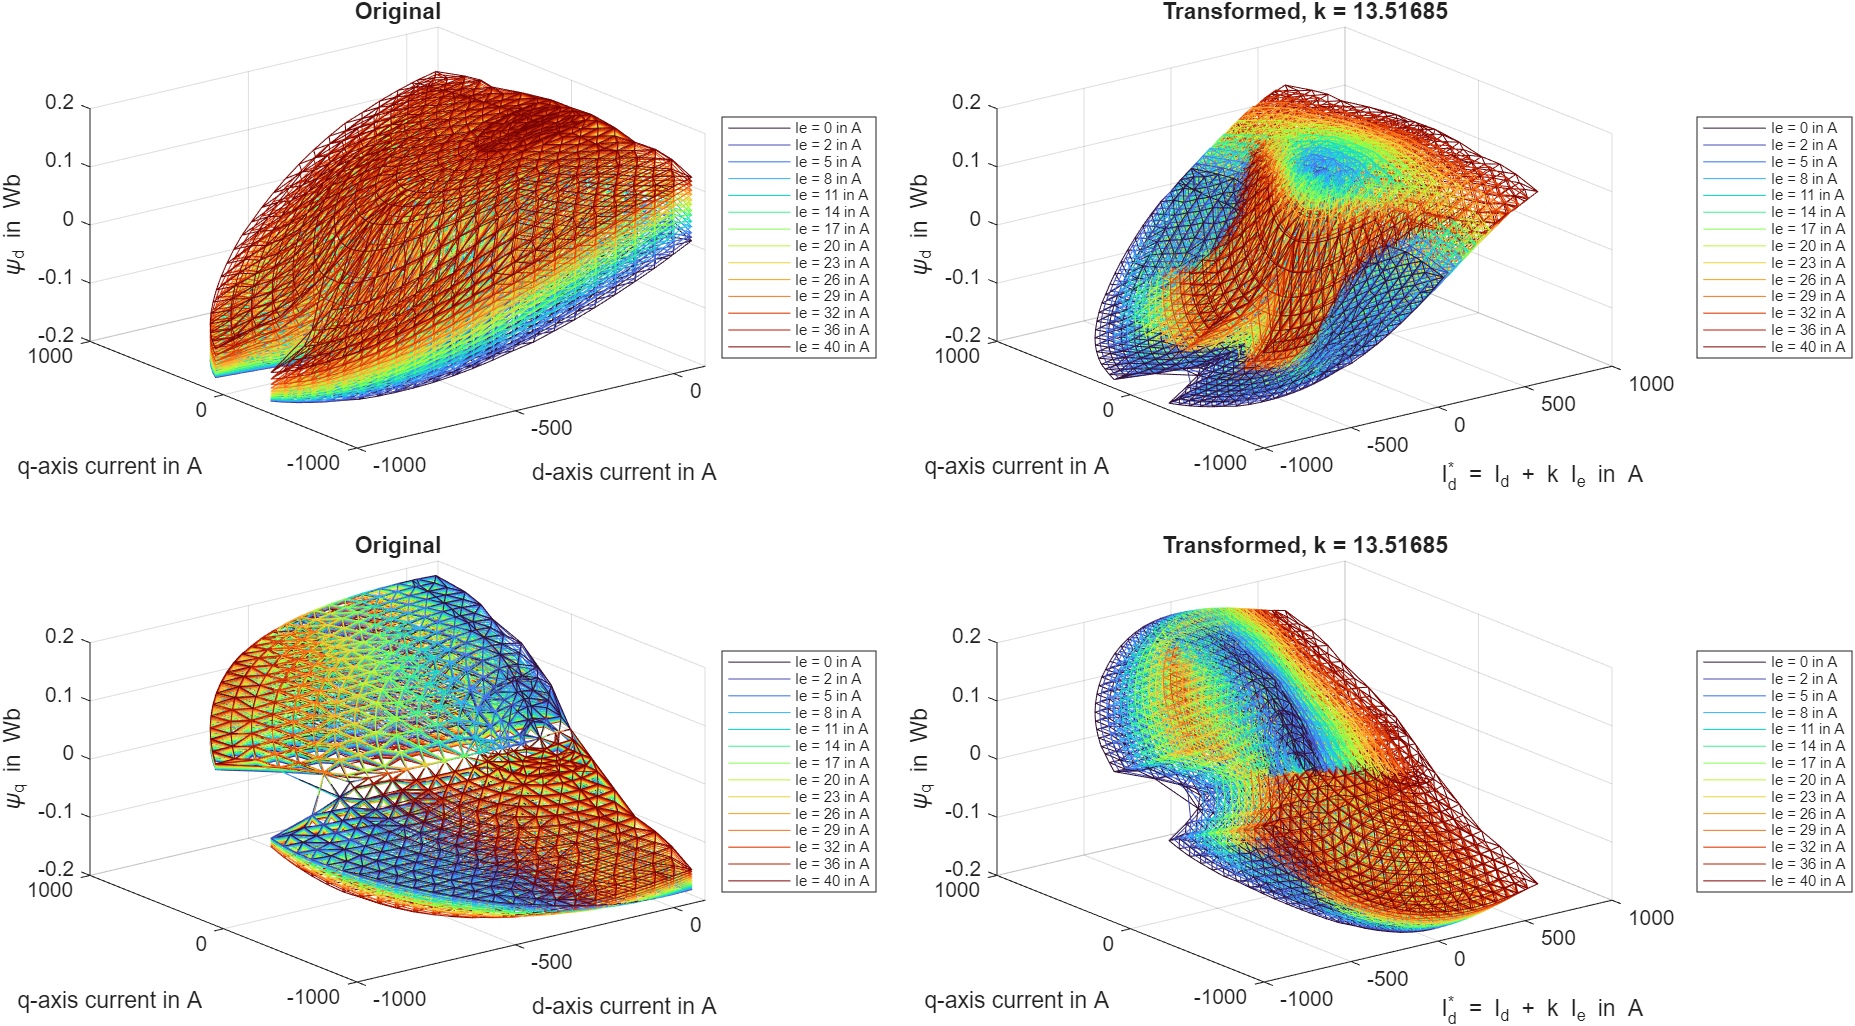
\includegraphics[width=\linewidth]{flux_original_transformed.png}
\caption{Set 2 original measured surfaces and the same flux values after the original constant coordinate shift. Color denotes nominal excitation current. This view shows geometry before evaluating a single merged approximation.}
\end{figure}
\begin{figure}[htbp]
\centering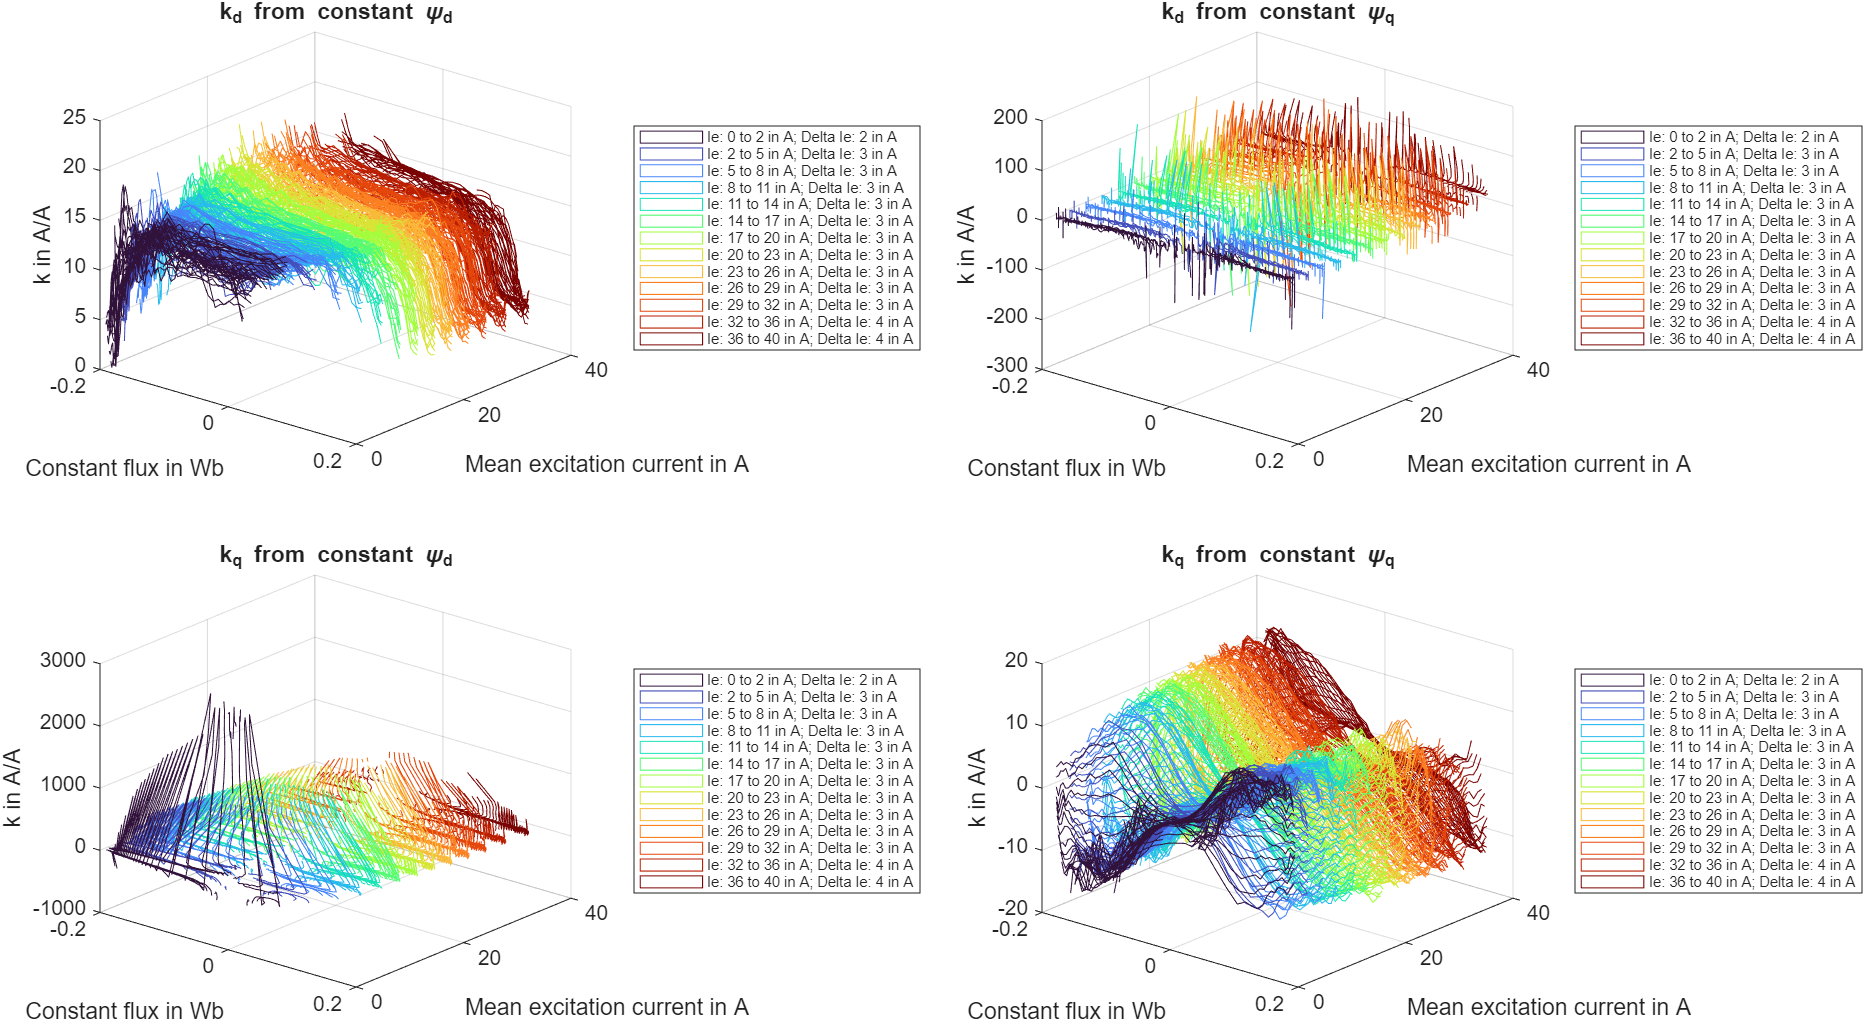
\includegraphics[width=\linewidth]{secants.png}
\caption{The four earlier finite-contour candidates, retained as exploratory views. Their midpoint assignment and secants are defined in Section~\ref{sec:contours}; they are not pointwise differential-inductance maps.}
\end{figure}

\clearpage
\begin{thebibliography}{9}
\bibitem{note}
User-supplied handwritten note, \emph{Motor Model}, three pages, Notability archive, supplied with this investigation.
\bibitem{turk}
N.~Turk, D.~Cika\v{c}, N.~Buli\'{c}, and S.~Barbanti,
\emph{A Novel Experimental Method for Identifying the Flux Linkage Map of a High-Power Medium-Voltage Electrically Excited Synchronous Machine with Double Stator Winding},
Machines, vol.~10, no.~3, article~187, 2022.
\url{https://doi.org/10.3390/machines10030187}.
\bibitem{matlab}
MathWorks, \emph{scatteredInterpolant: Interpolate 2-D or 3-D scattered data}, MATLAB documentation, accessed 23 October 2026.
\url{https://www.mathworks.com/help/matlab/ref/scatteredinterpolant.html}.
\end{thebibliography}

\end{document}

